% ------------------------------------------------------------------
% DOKUMENTEINSTELLUNGEN
% ------------------------------------------------------------------
\documentclass[
paper=a4,           % Page dimensions
fontsize=12pt,      % Schriftgröße 12 Punkt
DIV=12,             % Teilungsfaktor für Satzspiegel
listof=totoc,       % Tabellen & Abbildungsverzeichnis ins Inhaltsverzeichnis
bibliography=totoc, % Literaturverzeichnis ins Inhaltsverzeichnis
appendixprefix,   	% "Appendix" Prefix für Anhang
headinclude,        % Kopfzeile mit in Satzspiegel aufnehmen
twoside,            % Page margins for two-sided printing
open=right,         % Begin new chapters on a right-hand side
parskip,            % Space after last line of paragraph: 1em
draft=false,        % Draft version?
titlepage=on,       % Title at own page
fleqn,              % Formulas left-aligned
]{scrbook}          % oder {scrreprt}

% Alle Überschriften fett und *mit* Serifen (normale Schriftart und Größe)
\setkomafont{chapter}{\normalfont\bfseries\huge}
\setkomafont{section}{\normalfont\bfseries\Large}
\setkomafont{subsection}{\normalfont\bfseries\large}
\setkomafont{subsubsection}{\normalfont\bfseries}

% \usepackage{morewrites}
\usepackage{scrwfile}

% Repair some problems of komascript with other packages
\usepackage{scrhack}

% Custom page geometry
\usepackage{geometry}

\renewcommand{\textfraction}{0.01} % Minimum fraction of page for text
\renewcommand{\topfraction}{0.99} % Fraction of page from top that may contain figures
\renewcommand{\bottomfraction}{0.99} % Fraction of page from bottom that may contain figures
\renewcommand{\floatpagefraction}{0.99} % Avoid separate pages that only contain figures

% Page break before each section
\let\oldsection = \section
\renewcommand{\section}[1]{
  \clearpage
  \oldsection{#1}
}

% unterschiedliche linespaces (für die comments)
\usepackage{setspace}

% Handle page numbers on empty pages
\makeatletter
\def\cleardoublepage{\clearpage\if@twoside \ifodd\c@page\else
  \hbox{}
  \thispagestyle{empty} % no page number at empty pages
  % \thispagestyle{plain} % page number at empty pages
  \newpage
  \if@twocolumn\hbox{}\newpage\fi\fi\fi}
\makeatother

% ------------------------------------------------------------------
% ERWEITERUNGEN: SPRACHEINSTELLUNGEN
% ------------------------------------------------------------------

% Englische Spracheinstellung
% \usepackage[ngerman]{babel}
% Deutsche Spracheinstellung
\usepackage[ngerman]{babel}

% Kodierung
\usepackage[T1]{fontenc}
\usepackage[utf8]{inputenc}

% ------------------------------------------------------------------
% ERWEITERUNGEN: ALLGEMEIN
% ------------------------------------------------------------------

% Packages to allow inclusion of graphics
\usepackage{graphicx}
\usepackage{subcaption}
\usepackage{float}
\usepackage{caption}

% For creating coloured text and background
\usepackage[svgnames,rgb]{xcolor}

% Unformatierten Text einfügen
\usepackage{verbatim}

\usepackage{url}

% Einträge in PDF verlinken, keine Ränder
\usepackage{hyperref}

\hypersetup{
% bookmarks=true,                              % show bookmarks bar?
  bookmarksnumbered=true,
  pdftitle={Vergleich aktueller Implementierungen von Message Oriented Middlewares},                % title
  pdfauthor={Magnus Görlitz},                % author
  pdfsubject={Thesis},                   % subject of the document
  pdfkeywords={Modeling} {PubSub} {Message Broker}, % list of keywords
  colorlinks=true,                             % false: boxed links; true: colored links
  linkcolor=black,                             % color of internal links
  citecolor=red,                               % color of links to bibliography
  pdfborder={0 0 1}
}

% Provides a solution to the problem with hyperref that links
% to floats actually anchor to the place below the float's caption,
% instead of anchoring to the beginning of the float
\usepackage[all]{hypcap}

% EPS Grafiken einbinden
\usepackage{epstopdf}

% Decorative chapter headings | Muss nach xcolor geladen werden!
\usepackage[grey, utopia]{quotchap}

\usepackage{enumitem}

\usepackage{algorithm}
\usepackage[noend]{algpseudocode}

\usepackage{wrapfig} % Bilder mit Fließtext

\usepackage{tikz}


% ------------------------------------------------------------------
% ERWEITERUNGEN: ZITATE UND REFERENZEN
% ------------------------------------------------------------------

% Context sensitive quotation facilities
% Required by biblatex for multilingual quoting
\usepackage{csquotes}

% Use biblatex instead of bibtex -- it's the future.
\usepackage[
backend=biber,
natbib=true,        % Provide aliases for natbib's citation commands
citestyle=numeric,
style=numeric
]{biblatex}

\addbibresource{bibliography/references.bib}

% ------------------------------------------------------------------
% ERWEITERUNGEN: MATH
% ------------------------------------------------------------------

% Typical maths resource packages
\usepackage{amsmath,amssymb,amsfonts}

% Intelligent cross-referencing
\usepackage{cleveref}

% Mathematical typesetting with the Palatino fonts
\usepackage{mathpazo}

% Capital handwriting letters for mathematical purposes
% \usepackage{mathrsfs}

% Mathematical symbol font that contains symbol for disjoint union
\usepackage{MnSymbol}

% AMS theorems
\usepackage{amsthm}

\usepackage{framed}
% \usepackage[framed]{ntheorem}

% darstellung mathematischer definitionen
\usepackage{shadethm}


% ------------------------------------------------------------------
% ERWEITERUNGEN: TABLE
% ------------------------------------------------------------------

% Tables with variable column width
\usepackage{tabularx}

% Additional table commands for academic publications
\usepackage{booktabs}

% Rotate objects (used for vertical text in table cells)
\usepackage{rotating}

% Multilined table cells
\usepackage{makecell}

% Create tabular cells spanning multiple rows
\usepackage{multirow}

% Tables that span over several pages
\usepackage{longtable}

% ------------------------------------------------------------------
% ERWEITERUNGEN: VERZEICHNISSE
% ------------------------------------------------------------------

% Code-Listings
\usepackage{listings}
\lstset{
	basicstyle=\ttfamily\tiny,
	tabsize=2,
	breaklines=true,
	frame=single,
	captionpos=b,
	showstringspaces=false,
	numbers=left,
	numberfirstline=false,
	firstnumber=1,
	stepnumber=2,
	numbersep=5pt
  }
  
% Glossary
\usepackage[toc]{glossaries}
\makeglossaries
\loadglsentries{glossaries}

% ------------------------------------------------------------------
% KOPF-/FUSSZEILE
% ------------------------------------------------------------------
\renewcommand{\ttdefault}{lmtt} % bold texttt

% Use KOMA-recommended package for header/footer style setup
\usepackage[%
headsepline, % Trennlinie zwischen Inhalt und Kopfzeile
footsepline, % Trennlinie zwischen Inhalt und Fußzeile
automark     % Automatischer Inhalt von Seitenüberschriften
]{scrlayer-scrpage}

\usepackage{textcase} % for \MakeTextLowercase

\clearpairofpagestyles
\lehead{\MakeTextLowercase{\textsc{\leftmark}}}
\rohead{\MakeTextLowercase{\textsc{\rightmark}}}
\ofoot{\pagemark}

% Abstand zwischen Kopf-/Fußzeile und Trennlinie
\chead{\rule[-\dimexpr \dp\strutbox+1ex\relax]{0pt}{\baselineskip}}
\cfoot{\rule[-\dimexpr \dp\strutbox+1ex\relax]{0pt}{\baselineskip}}

\addtokomafont{pageheadfoot}{\small\textcolor{gray!85}}
\setkomafont{pagenumber}{\small\textcolor{gray!85}}

% Separator line for headers/footers
\KOMAoptions{headsepline=.4pt:\textwidth}
\KOMAoptions{footsepline=.4pt:\textwidth}

\setkomafont{headsepline}{\color{gray!75}}
\setkomafont{footsepline}{\color{gray!75}}


% beamer-style shaded text box with title
\usepackage{tcolorbox}
\usetikzlibrary{shadings,shadows}

\newenvironment{frameblock}[1]{%
  \tcolorbox[beamer,%
  noparskip,breakable,
  colback=LightGray,colframe=DarkGray,%
  colbacklower=DarkBlue!75!LightBlue,%
  title=#1]}%
{\endtcolorbox}

\newenvironment{frameblockk}[1]{%
  \tcolorbox[beamer,%
  noparskip,breakable,width=0.7\textwidth,
  colback=LightGray,colframe=DarkGray,%
  colbacklower=DarkBlue!75!LightBlue,%
  title=#1]}%
{\endtcolorbox}
\usepackage{fancybox}
% ------------------------------------------------------------------
% KOMMANDOS
% ------------------------------------------------------------------
% Informationen ------------------------------------------------------------
% 	Definition von globalen Parametern, die im gesamten Dokument verwendet
% 	werden können (z.B auf dem Deckblatt etc.).
% --------------------------------------------------------------------------

% Allgemeine Informationen
\title{Vergleich aktueller Implementierungen von Message Oriented Middlewares}
% \subtitle{and its applications}
\author{Magnus Görlitz}
\newcommand{\place}{Augsburg}

\newcommand{\art}{Thesis}
\newcommand{\degreetext}{for the degree of}
\newcommand{\degree}{Bachelor of Science (B.Sc.)}
\newcommand{\universitaet}{University of Augsburg}
\newcommand{\institut}{Department of Computer Science}
\newcommand{\professur}{Software Methodologies for Distributed Systems}

\newcommand{\monat}{February}
\newcommand{\jahr}{2019}

\newcommand{\monatV}{*MonthDefense*}
\newcommand{\jahrV}{2019}

\newcommand{\gutachtereins}{\textbf{Prof.~Dr.~Bernhard Bauer}, Department of Computer Science,}
\newcommand{\gutachterzwei}{\textbf{Prof.~Dr.~Bernhard Möller}, Department of Computer Science,}
\newcommand{\gutachterinst}{University of Augsburg, Germany}
%\newcommand{\gutachterdrei}{Prof.~Dr.~Severus Snape (University of Hogwarts)}

% Farben
\definecolor{lightgray}{gray}{0.95}
\definecolor{darkgray}{gray}{0.3}


% Abkürzungen
\newcommand{\vgl}{Vgl.\ }
\newcommand{\ua}{\mbox{u.\,a.\ }}
\newcommand{\zB}{\mbox{z.\,B.\ }}
%%% Local Variables:
%%% mode: latex
%%% TeX-master: "../TemplateSMDS"
%%% End:

% --------------------------------
% Neue global benutzbare Kommandos
% --------------------------------
\newcommand\insertemptypage{%
  \newpage
  \thispagestyle{empty}
  \mbox{}
}

% description in enum lists
\newcommand\litem[1]{\item{\bfseries #1\\}}

% =======================================================================
% TIKZ
% =======================================================================

\newcommand*\circled[1]{\tikz[baseline=(char.base)]{%
    \node[shape=circle,draw,minimum size=4mm,inner sep=0pt] (char) {#1};}}
\providecommand{\csnode}[1]{\circled{#1}}

\newcommand*\circledf[1]{\tikz[baseline=(char.base)]{%
    \node[shape=circle,draw,fill=black,minimum size=5mm,inner sep=0pt] (char) {#1};}}
\providecommand{\csnodef}[1]{\circledf{\color{white} #1}}


\newcommand{\csrect}[2][]{%
  \tikz[baseline=(char.base)] \node [shape=rectangle, draw=black, inner sep=1pt, rounded corners, minimum size=4mm,#1] {#2};%
}

% =======================================================================
% Layout / Struktur
% =======================================================================

\newcommand{\marginlabel}[1]{\mbox{}\marginline{\hspace{0pt}\RaggedRight\footnotesize #1}}

% Neue Zeile erzwingen (z.B. für 'description' Umgebung)
\newcommand\fnl{\textcolor{white}{\\}}

% Kleine Überschrift
\newcommand\subpar[1]{\vspace{15pt} \textbf{#1}\vspace{10pt} \\}

% Zentrierte, farbig hinterlegte Textbox
\newcommand\textbox[1]{%
  \vspace*{2mm}
  \begin{center}
    \fcolorbox{darkgray}{lightgray}
    {
      \parbox{0.80\textwidth}
      {
        \begin{flushleft}
          #1
        \end{flushleft}
      }
    }
  \end{center}
  \vspace*{2mm}
}

% Nicht zentrierte, farbig hinterlegte Textbox
\newcommand\textboxnc[1]{%
  \vspace*{2mm}
  \fcolorbox{darkgray}{lightgray}
  {
    \parbox{0.60\textwidth}
    {
      \begin{flushleft}
        #1
      \end{flushleft}
    }
  }
  \vspace*{2mm}
}

% Nicht zentrierte, farbig hinterlegte Textbox
\newcommand\textboxm[2]{%
  \vspace*{2mm}
  \fcolorbox{darkgray}{lightgray}
  {
    \parbox{#1\textwidth}
    {
      \begin{flushleft}
        #2
      \end{flushleft}
    }
  }
  \vspace*{2mm}
}

% Nicht zentrierte, farbig hinterlegte Textbox
\newcommand\textboxdfa[1]{%
  \vspace*{2mm}
  \fcolorbox{darkgray}{lightgray}
  {
    \parbox{0.45\textwidth}
    {
      \begin{flushleft}
        #1
      \end{flushleft}
    }
  }
  \vspace*{2mm}
}

\makeatletter
\newcommand{\paragr}[1]{\@startsection{paragraph}{4}{\z@}%
  {-3.25ex\@plus -1ex \@minus -.2ex}%
  {1.5ex \@plus .2ex}
  {\normalfont\normalsize\bfseries}}
\makeatother

% =======================================================================
% Mathematik
% =======================================================================

\providecommand{\abs}[1]{\lvert#1\rvert}
\providecommand{\Abs}[1]{\left\lvert#1\right\rvert}
\providecommand{\norm}[1]{\left\Vert#1\right\Vert}
\providecommand{\Trace}[1]{\ensuremath{\Tr\{\,#1\,\}}} % Trace /Spur

% -- Sets of numbers -- 
\newcommand{\nat}{\mathbb{N}}     % Integers
\newcommand{\rat}{\mathbb{Q}}     % Rationals
\newcommand{\complex}{\mathbb{C}} % Complex numbers
\newcommand{\real}{\mathbb{R}}    % Real numbers


\RequirePackage[ngerman=ngerman-x-latest]{hyphsubst}
\usepackage[graphicx]{realboxes}

% ------------------------------------------------------------------
% DOKUMENT
% ------------------------------------------------------------------
% Verwendet von: (Abstract, erste Seite eines Kapitels, Verzeichnisse, Leerseiten)

\begin{document}

\newshadetheorem{challenge}{Challenge}[section]

% standard definition theorem
% \theoremstyle{definition}
\newshadetheorem{defs}{Definition}[section]

% \newmdtheoremenv[
%    hidealllines=true,
%    innerleftmargin=4pt,%
%    innerrightmargin=10pt,%
%    innertopmargin=4pt,%
%    innerbottommargin=4pt,%
%    backgroundcolor=gray!10,%
%    skipbelow=\baselineskip,%
%    skipabove=\baselineskip]{defs}{Definition}[section]
% \crefname{defs}{Definition}{Definitions}
 
%\theoremstyle{corollary}
\newshadetheorem{cors}[defs]{Corollary}

\setcounter{secnumdepth}{3}
\definecolor{shadethmcolor}{rgb}{.97,.97,.97}   % Farbe des Hintergrundes 

% \theoremstyle{plain}
% \theoremsymbol{\ensuremath{\clubsuit}}
% \theoremseparator{.}
% \theoremprework{\bigskip\hrule}
% \theorempostwork{\hrule\bigskip}
% \newtheorem{Definition}{Definition}



% ------------------------------------------------------------------
% FRONT
% ------------------------------------------------------------------

\pagenumbering{roman}\setcounter{page}{1}
%\pagestyle{plain}

% ------------------------------------------------------------------------------------------------------
% TITLE
% ------------------------------------------------------------------------------------------------------

\makeatletter
\begin{titlepage}
  \newgeometry{top=30mm,bottom=30mm,right=30mm,left=30mm}
  \centering
  % \vspace*{\fill}
  \huge
  \textsc{\@title}\par
  \LARGE\@subtitle
  \vspace*{10mm}

  \LARGE{\@author}

  \vspace*{10mm}

  \LARGE{\textsc{\art}}\\

  \large{%
    \degreetext\\
    \degree}

  \vspace*{10mm}

  
\includegraphics[height=40mm]{figures/uni_siegel}

  \vspace*{5mm}

  \large
  \universitaet\\
  \vspace*{2mm}
  \institut\\
  \vspace*{2mm}
  \professur\\
  \vspace*{5mm}

  \monat~\jahr
  
  \vspace*{\fill}
  
\includegraphics[width=.4\paperwidth]{figures/logo_CHECK24_transparent.png}
  
\includegraphics[width=.4\paperwidth]{figures/logo_SMDS_transparent.png}
\end{titlepage}

\restoregeometry
\thispagestyle{empty}
\vspace*{\fill}
\textbf{\@title}
\begin{tabbing}
  \hspace*{4cm}\=\hspace*{12cm}\= \kill
  Erstprüfer: \> \textbf{Prof.~Dr.~Bernhard~L.~Bauer}, Department of Computer Science,\\
	\> University of Augsburg, Germany\\[2mm]
	Zweitprüfer: \> \textbf{Prof.~Dr.~Bernhard~Möller}, Department of Computer Science,\\
  \> University of Augsburg, Germany\\[2mm]
  Betreuer: \> \textbf{M.Sc.~Melanie~Langemeier}, Department of Computer Science,\\
  \> University of Augsburg, Germany\\[2mm]
  Firmenbetreuer: \> \textbf{M.Sc.~Fabian~Zintgraf}, Team Lead IT,\\
  \> CHECK24 Versicherungsservice GmbH, Germany\\[2mm]
\end{tabbing}

Copyright \copyright\ \@author, \place, \monat~\jahr
\makeatother

%%% Local Variables:
%%% mode: latex
%%% TeX-master: "TemplateSMDS"
%%% End:

% ------------------------------------------------------------------------------------------------------
% TABLE OF CONTENTS
% ------------------------------------------------------------------------------------------------------
%%%%%%%%%%%%%%%%%%%%%%%%%%%%%%%%%%%%%%%%%%%%%%%%%%%%%%%%%%%%%%%%%%%%%%%%%%%%%%%%
%%%%%%%%%%%%  Abstract
%%%%%%%%%%%%%%%%%%%%%%%%%%%%%%%%%%%%%%%%%%%%%%%%%%%%%%%%%%%%%%%%%%%%%%%%%%%%%%%%
\chapter*{Kurzbeschreibung}
% was, warum?
In der modernen Softwareentwicklung finden sich in großen Anwendungen häufig
sogenannten \textit{Message Oriented Middlewares} wieder. Hierbei handelt es sich
um Systeme, die eine effiziente Kommunikation zwischen einer großen Anzahl
von Prozessen ermöglichen, oft auch in verteilten Systemen oder heterogenen
Netzen. In den letzten Jahren gab es vermehrt Weiterentwicklungen im Bereich
der Message Oriented Middleware, da diese nicht zuletzt auch in Microservices
vermehrte Verbreitung gefunden haben.
Hierbei handelt es sich um Message Oriented Middlewares, die als eigene
Anwendung unabhängig vom restlichen System betrieben werden.
Es existieren viele Implementierungen, wobei sich diese untereinander
stark unterscheiden können.
Bei der Konzeption eines Systems, welches eine Message Oriented Middleware verwendet, 
verliert man daher schnell den Überblick über diese.

% arbeit
Aus diesem Grund wird diese Arbeit einen Überblick über bestehende Lösungen geben und diese
auf konzeptioneller Ebene vergleichen. Einzelne Punkte, in denen sich diese
unterscheiden, werden dabei begründet erarbeitet und zu einem Katalog
zusammengefasst werden. 
Dies ermöglicht, die Erkenntnisse aus der Arbeit
auch auf zukünftige Entwicklungen anzuwenden.
Daraufhin wird ein Vergleich erstellt, um die aktuell führenden Implementierungen aufzeigen
und ihre Unterschiede in den Punkten dieses Kataloges gegenüberzustellen. 
Letztendlich soll für ein Zielsystem des Betreuers
(CHECK24 Versicherungsservice GmbH) eine geeignete Implementierung
gewählt werden. Da die Umsetzung den Rahmen der Arbeit sprengen würde, wird
sich hier auf eine Analyse der möglichst optimalen Lösungen beschränkt.
Hierzu werden für dieses System spezifische Anforderungen identifiziert und
versucht, mit dem im zweiten Teil der Arbeit vorgestellten Katalog eine 
Kategorie für dieses Zielsystem zu finden. Daraufhin kann eine Empfehlung einer Lösung ausgesprochen
werden. Da eine konkrete Implementierung entfällt, werden theoretische Probleme
der empfohlenen Implementierung erörtert und Lösungsvorschläge präsentiert werden.
% Wozu -> Forschungsfragen

Zusammenfassend wird zum einen ein Überblick über Implementierungen erstellt,
der diese konkret vergleicht. Dabei werden einzelne Punkte des Vergleichs vorher
erarbeitet und anschließend nach Relevanz eingeordnet. Letztendlich werden
anhand eines Fallbeispiels die vorherigen Abschnitte validiert und ein Fazit
gezogen.

\chapter*{Danksagung}
An dieser Stelle möchte ich meinem Firmenbetreuer Fabian Zintgraf danken,
der maßgeblich zur Inspiration der Arbeit beigetragen und mich stets unterstützt hat.
Der Austausch über die Inhalte meiner Arbeit mit ihm und dem Team des CHECK24
Versicherungscenters waren von unschätzbarem Wert.

\cleardoublepage
\tableofcontents
\cleardoublepage
 
% ------------------------------------------------------------------------------------------------------
% ABSTRACT
% ------------------------------------------------------------------------------------------------------
\pagenumbering{arabic}\setcounter{page}{1}
\chapter{Einführung}
\label{intro:einleitung}
%%%%%%%%%%%%%%%%%%%%%%%%%%%%%%%%%%%%%%%%%%%%%%%%%%%%%%%%%%%%%%%%%%%%%%%%%%%%%%%%
%%%%%%%%%%%%  Acknowledgements
%%%%%%%%%%%%%%%%%%%%%%%%%%%%%%%%%%%%%%%%%%%%%%%%%%%%%%%%%%%%%%%%%%%%%%%%%%%%%%%%
\section{Motivation}
\label{intro:motivation}
In der CHECK24 Versicherungsservice GmbH kommen im 
\textit{Versicherungscenter}\footnote{https://www.check24.de/versicherungscenter/,
abgerufen am 23.11.2018} im Laufe des Jahres neue Businessanforderungen auf die
vorhandene Infrastruktur zu. Im Rahmen der Neuerungen wurde erwogen, eine
Message Oriented Middleware in das System zu integrieren. Dabei reichten jedoch
die Erfahrungen anderer Teams nicht aus, um eine Entscheidung bezüglich der
konkreten Implementierungen zu fällen.

Die konkreten Anforderungen waren zu unterschiedlich zu denen von anderen Teams, um
von Ihren Erfahrungen sinnvolle Schlüsse ableiten zu können. Daher soll eine
Evaluierung der Optionen stattfinden, was den Anreiz für diese Arbeit gab. Es soll
also nicht nur eine Analyse und ein Vergleich von marktführenden
Lösungen stattfinden, sondern auch in einem Praxisteil das konkrete Szenario
untersucht und eine Empfehlung ausgesprochen werden.

Der bis dahin aufgestellte Eigenschaftenkatalog und die Analyse existierender
Implementierungen sollen helfen, eine fundierte Wahl einer Lösung zu treffen. Zudem
sollen die erarbeiteten Grundlagen Missverständnisse vorbeugen und zum Verständnis
bei der Integration beitragen.

%%%%%%%%%%%%%%%%%%%%%%%%%%%%%%%%%%%%%%%%%%%%%%%%%%%%%%%%%%%%%%%%%%%%%%%%%%%%%%%%
%%%%%%%%%%%%  Introduction
%%%%%%%%%%%%%%%%%%%%%%%%%%%%%%%%%%%%%%%%%%%%%%%%%%%%%%%%%%%%%%%%%%%%%%%%%%%%%%%%
\section{Problemstellung}
\label{intro:problem}
Um einen möglichst universellen Vergleich zwischen Message Oriented Mid\-dlewares
zu ermöglichen, muss der Begriff zuerst umfangreich definiert werden.
Nur auf dieser Grundlage ist eine Gegenüberstellung von Implementierungen sinnvoll.

Weiter soll der Vergleich aufgrund ausgewählter, wichtiger Eigenschaften
von Message Oriented Middlewares geschehen.
Diese müssen also erarbeitet und anhand Ihrer Relevanz eingeschätzt werden.
Dabei können Eigenschaften beliebig detailliert oder abstrakt sein.
Es besteht also eine Herausforderung da\-rin, ein geeignetes Abstraktionslevel zu
finden. Anschließend soll dieser Eigenschaftenkatalog anhand eines Praxisteils
evaluiert werden.

Eine weitere Herausforderung besteht im Vergleich bestehender Message Oriented
Middlewares. Es sollte aus den verbreiteten Lösungen eine repräsentative Menge
ausgewählt werden. Also eine Menge, die einerseits groß genug ist, um genug
verschiedene Repräsentanten zu beinhalten, andererseits aber klein genug ist,
um noch übersichtlich und relevant zu sein. 

Somit sollten die Vergleichspunkte fundiert erarbeitet und nach Relevanz
bewertet werden. Letztendlich sollte der Anspruch sein, eine realistisch nutzbare
Orientierung bei der Planung eines Systems zu erstellen.
Dementsprechend sind die grundlegenden Herausforderungen dieser Arbeit die
Erarbeitung eines Eigenschaftenkatalogs und die Analyse einzelner ausgewählter
Implementierungen damit, sowie die Anwendung und Evaluierung anhand eines
Praxisbeispiels.

%\insertemptypage

% ------------------------------------------------------------------
% MAIN MATTER
% ------------------------------------------------------------------


% ------------------------------------------------------------------------------------------------------
% PART I
% ------------------------------------------------------------------------------------------------------
\cleardoublepage
\label{part:Message Broker}
\chapter{Grundlagen}
% In diesem Abschnitt werden Message Broker behandelt.
% Dabei wird erst ein Überblick über die grundlegende Funktionsweise von
% Message Brokern verschafft. Anschließend soll der Begriff abgegerenzt werden.
% Es werden des Weiteren Anwendungsszenarien für Message Broker beschrieben.
% Auch die mit ihnen einhergehenden Probleme und Herausforderungen werden beschrieben.

\section{Definition}
\label{definition:definition}
\subsection{Message Oriented Middleware}
Eine \textit{Message Oriented Middleware} (kurz MOM), also eine
nachrichtenorientierte Middleware, wird definiert als eine beliebige Middleware,
die es ihren \textit{Clients} ermöglicht, Nachrichten aneinander zu versenden \cite{tanenbaum2007distributed}.
Diese entkoppelt Sender und Empfänger (in diesem Kontext auch
\textit{Producer} und \textit{Consumer} genannt \cite{eugster2003many}), da nun nicht
mehr alle Teilnehmer untereinander verbunden sein müssen, sondern nur noch mit
der Middleware.
Dies wird in den Darstellungen \ref{Message Broker:rpcvsmom} abgebildet.
Hierbei wird in beiden Fällen die Netzwerkarchitektur gezeigt, die benötigt wird,
damit jeder Teilnehmer an jeden anderen Teilnehmer Nachrichten senden kann.
Dargestellt sind Clients bzw. bei (b) Clients und in der Mitte eine MOM.

Dabei beschreibt der Begriff Message Oriented Middleware keine konkrete Umsetzung.
Eine solche besteht in den meisten modernen Implementierungen aus einem oder
mehreren Brokern, die nach einem gewissen Schema routen sowie Queues, die
Nachrichten speichern können. Diese Strukturen werden in den nächsten Abschnitten
detailliert erklärt. \cite{curry2004message}

\begin{figure}[h]
  \centering
  \begin{subfigure}{.49\textwidth}
    \centering
    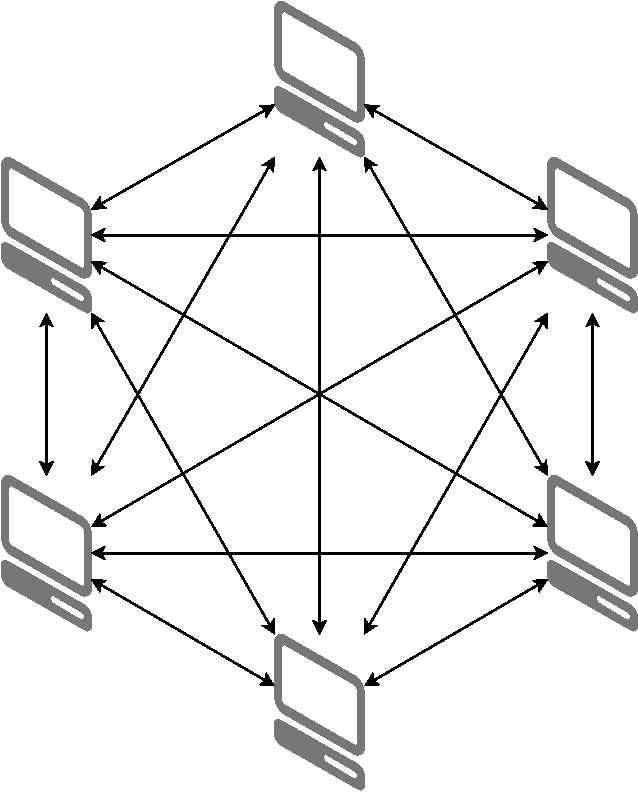
\includegraphics[width=0.5\textwidth]{figures/rpc.pdf}
    \caption{Aufbau ohne MOM}
    \label{Message Broker:rpcvsmom:rpc}
  \end{subfigure}
  \begin{subfigure}{.49\textwidth}
    \centering
    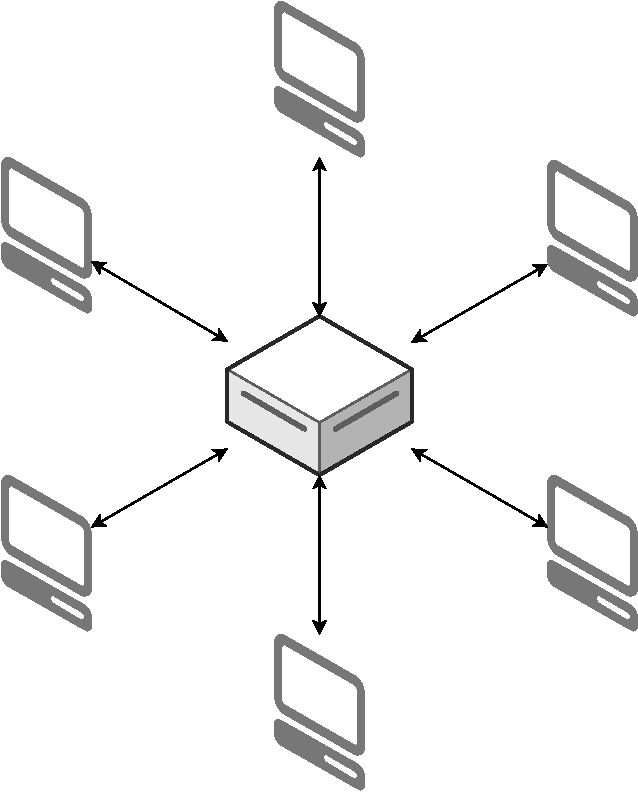
\includegraphics[width=0.5\textwidth]{figures/broker.pdf}
    \caption{Aufbau mit MOM}
    \label{Message Broker:rpcvsmom:mom}
  \end{subfigure}
  \caption{Netzwerkarchitektur bei Verwendung direkter Kommunikation im Vergleich mit einer Message Oriented Middleware}
  \label{Message Broker:rpcvsmom}
\end{figure}

Ein \textit{Message Broker} sorgt für das Weiterleiten der Nachrichten an den
richtigen Empfänger. Dabei kann er auch Nachrichten, die in
einem bestimmten Format angenommen wurden, in ein anderes, zum Empfänger
kompatibles Format umwandeln. Er sorgt also für eine Entkopplung von
Nachrichtenformaten.
Bei der Verwendung eines Brokers werden alle Nachrichten über diesen geleitet. 
Er verarbeitet die Nach\-richten und leitet sie nach gewissen Regeln weiter.
Man spricht auch von einem \textit{Routing}, hierauf wird in Abschnitt 
\ref{definition:routing} näher eingegangen. \cite{tanenbaum2007distributed}

Eine Queue ist im Kontext von MOM eine Speicherlösung für Nachrichten.
Dabei können je nach Implementierung eine oder mehrere Queues für die gesamte
MOM existieren. Auch ob eine Queue vor den
Message Broker geschaltet wird, oder dieser seine Nachrichten an eine Queue
weiterleitet, ist implementierungsabhängig \cite{KafkaClients:online,RabbitMQ:online}.
Warum Queues verwendet werden und welche Vorteile dies haben kann, wird in
Abschnitt \ref{definition:queues} besprochen.
Eine Veranschaulichung eines exemplarischen Gesamtaufbaus einer MOM mit den
eben besprochenen Teilen ist in Darstellung \ref{definition:momfigure} zu finden.
Hierbei ordnet der Message Broker die empfangenen Nachrichten in eine der Queues
ein, von denen die Consumer diese erhalten.

\begin{figure}[h]
  \centering
    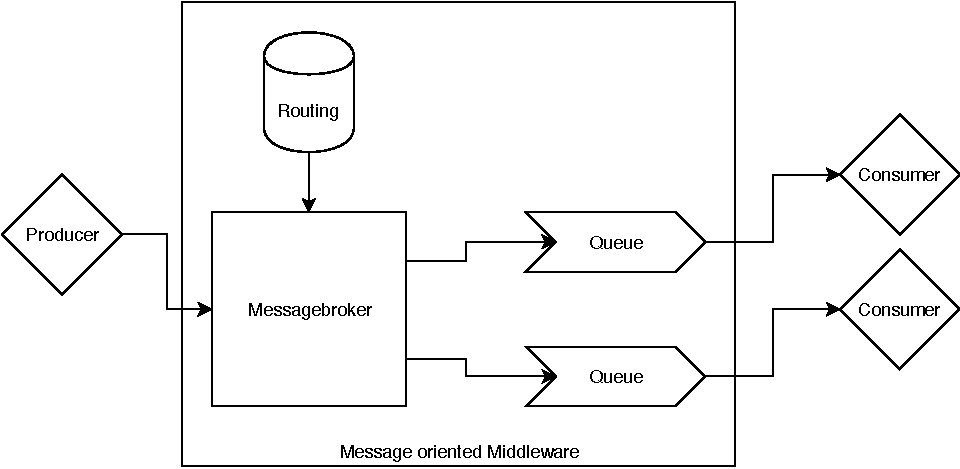
\includegraphics[width=0.9\textwidth]{figures/mom.pdf}
  \caption{Exemplarischer Aufbau einer Message Oriented Middleware}
  \label{definition:momfigure}
\end{figure}

Ein großer Vorteil, den eine MOM bieten kann, ist \textit{asynchrone} Kommunikation.
Ist eine Architektur synchron, so wird bei dem Verschicken der
Nachricht der weitere Ablauf des Senders blockiert, bis eine Antwort erhalten
und der Ablauf fortgesetzt wird. Bei der asynchronen Variante kann eine
Nachricht verschickt werden, ohne dass der Ablauf dadurch blockiert wird.
Dies ist vor allem in Batchverarbeitungs- und parallelen Systemen nützlich \cite{tanenbaum2007distributed}.
Zur Veranschaulichung dient Abbildung \ref{Message Broker:communication}, in
der der asynchrone Versand einer Nachricht dargestellt ist. Dabei wird die erste
Nachricht von \textit{Client 2} verarbeitet und danach eine Antwort verschickt.
Weitere Vorteile werden in Abschnitt \ref{Message Broker:advantages} besprochen.

In den untersuchten Implementierungen findet dabei das \textit{Publish-Subscribe}
Pattern Anwendung. Es beschreibt die Art, wie sich zwei verschiedene Teile einer
Software miteinander verbinden und kommunizieren. Dabei ist bei Publish-Subscribe
(kurz auch PubSub) eine Nachricht nicht an einen Empfänger direkt gerichtet,
sondern Sender können Nachrichten veröffentlichen (publish) und interessierte
Empfänger können ihr Interesse durch eine Subscription bekunden.
Daraufhin erhalten alle Subscriber, beispielsweise eines bestimmten Themas, alle
Nachrichten davon. Auf welche Art diese Auswahl stattfindet, wird genauer im nächsten
Abschnitt (\ref{definition:routing} Routing) beschrieben. \cite{eugster2003many}

\begin{figure}[h]
  \centering
    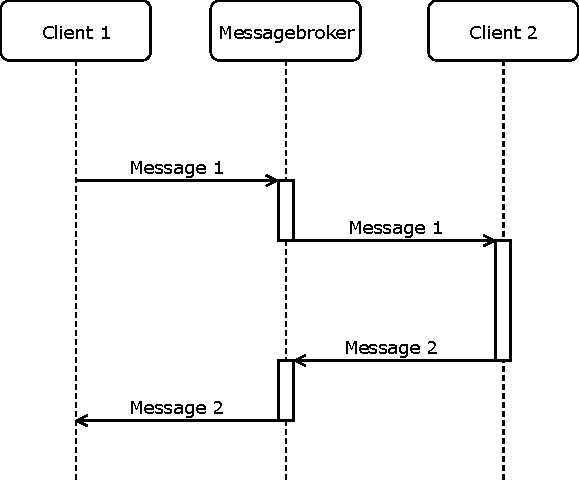
\includegraphics[width=0.5\textwidth]{figures/communication.pdf}
  \caption{Asynchrone Kommunikation mithilfe eines Message Brokers}
  \label{Message Broker:communication}
\end{figure}

\subsection{Routing}
\label{definition:routing}
Message Broker müssen architekturbedingt ein Regelwerk anbieten, nach dem Nachrichten
bestimmten Empfängern zugestellt werden, da die Nachrichten nicht direkt an diese
geschickt werden. Man spricht von einem \textit{Routing}.
So kann man neben statisch festgelegten Routen auch \textit{Channel-},
\textit{Topic-}, oder \textit{Content-}basiert geroutet werden \cite{tanenbaum2007distributed}.
Bei channelbasiertem Routing werden Kanäle gebildet, denen Clients beitreten können;
daraufhin erhalten diese alle in dem Kanal veröffentlichten Nachrichten.
Eine weitere Möglichkeit ist das Bilden von \textit{Topics}, wodurch dann je
nach thematischer \textit{Subscription} des einzelnen Clients Nachrichten zugestellt werden
\cite{eugster2003many}.
Bei inhaltsbasiertem Routing wird basierend auf dem Inhalt der einzelnen Messages vom
Broker beurteilt, welche Consumer diese erhalten \cite{tanenbaum2007distributed}.

Dabei sind je nach Protokoll und Implementierung verschiedene Ausprägungen anzutreffen.
Die meisten bieten mindestens eine Topic-Logik, oft auch eine Bildung von Channels an.
Sie unterscheiden sich hauptsächlich darin, wie mit mehreren Topics umgegangen wird.
Es können beispielsweise Wildcards verwendet oder logische Verknüpfungen
erstellt werden.
Wenn z.B. gewünscht ist, dass ein Consumer alle Topics der Nachricht 
abonniert haben muss, um diese zu erhalten, kann dies unter anderem mit
RabbitMQ bzw. dem verwendeten AMQP-Protokoll realisiert werden \cite{dobbelaere2017kafka}.
Weitere Details zu den jeweiligen Routingoptionen werden im Abschnitt
\ref{part:comparison} für die einzelnen Implementierungen besprochen.

\subsection{Queues}
\label{definition:queues}
Um eine stärkere Entkopplung zu erreichen, werden in modernen Implementierungen
häufig Queues verwendet.
Im Kontext von Message Oriented Middleware sind hier mit Queues
Speicher für Nachrichten gemeint \cite{curry2004message}.
Je nach Implementierung wird eine Nachricht hier nur zwischengespeichert, bis
sie erfolgreich weitergeleitet wurde, oder dauerhaft gespeichert.
Dies hat zwei Vorteile. Zum einen können bei einer langsamen Abarbeitung von
den Consumern die Nachrichten zwischengespeichert werden, und gehen nicht verloren.
Zum anderen kann eine langfristige Speicherung beispielsweise als Backup fungieren.
Dabei stößt man auf die üblichen Prinzipien von Warteschlangen. Im Kontext von
nachrichtenorientierten Middlewares ist eine Queue meistens ein \textit{FIFO},
gibt also die Nachrichten nach dem Zwischenspeichern in unveränderter Reihenfolge
wieder an den Empfänger aus \cite{curry2004message}.
Es existieren jedoch Lösungen wie Kafka, bei denen zwar eine Ordnung innerhalb
einzelner Queues vorliegt, jedoch die Broker zusätzlich zu ihrer normalen
Publish-Subscribe Kommunikation auch gezielt beliebige gespeicherte Nachrichten
abrufen können. Hierbei kann also nicht nach üblichen Kriterien von
Warteschlangen bewertet werden \cite{ApacheKa84:online}.
Wie bereits erwähnt, ist es abhängig von der Implementierung, wie die Queue
mit dem Rest der MOM zusammenarbeitet. Details hierzu werden im Abschnitt
\ref{part:comparison} für die jeweilige Implementierung besprochen.

\subsection{Protokolle}
Je nach Implementierung werden verschiedene Protokolle verwendet und unterstützt.
Dabei existieren komplett proprietäre Protokolle bzw. Eigenentwicklungen, wie zum
Beispiel bei ZeroMQ oder Kafka \cite{ApacheKa84:online}. 
Abseits hiervon hat sich vorerst vor allem \textit{JMS}, das Java Message
Service Protokoll, durchgesetzt. Dies wird in ActiveMQ, JBOSS Messaging und
einigen anderen Implementierungen verwendet \cite{dobbelaere2017kafka}.
Als populäres und standardisiertes Protokoll ist auch \textit{AMQP},
Advanced Message Queueing Protocol, hervorzuheben \cite{vinoski2006advanced}.
Es findet in RabbitMQ, Qpid, HornetMQ und Weiteren Verwendung \cite{dobbelaere2017kafka}.
Daneben gibt es noch weitere Protokolle wie NMS, STOMP und WebSocket, allerdings
wird in der Industrie hauptsächlich AMQP verwendet. \cite{vinoski2006advanced}
Erwähnenswert ist jedoch noch MQTT (Message Queue Telemetry Transport), ein
im IoT-Bereich weit verbreitetes Protokoll. Es zeichnet sich durch seine
Leichtgewichtigkeit und einfache Implementierung aus \cite{dobbelaere2017kafka}.

AMQP ist ein offener Standard, um Nachrichten zwischen zwei Anwendungen
auszutauschen. 
Es wurde durch eine Arbeitsgruppe zusammengestellt und Anfang 2010 in seiner
ersten Version präsentiert.
Um von der großen Verbreitung von JMS profitieren zu können, wurde für Kompatibilität
gesorgt \cite{vinoski2006advanced}. Somit kann AMQP auch in einer JMS-Umgebung
integriert werden, um von AMQPs erhöhter Kompatibilität mit weiterer Software
profitieren zu können.
AMQP legt fest, wie die Kommunikation zwischen den Clients und den Brokern abläuft,
jedoch nicht, was der Broker tut. Daher können verschiedene Broker untereinander
unterschiedliche Funktionalitäten zur Verfügung stellen und trotzdem AMQP
unterstützen.

Die meisten Protokolle sind Netzwerkprotokolle und arbeiten auf der Anwendungsebene.
Sie umfassen dabei Spezifizierungen darüber, wie die Nachrichten verschickt werden.
Im Falle von AMQP wurde dies mit einem binären Peer-to-Peer Protokoll umgesetzt.
Weiter wird meistens ein bestimmtes Nachrichtenformat vorgegeben, nach denen alle
in der MOM propagierten Nachrichten strukturiert sind. Hierbei liegen auch die
Unterschiede in Protokollen, da sie erstens noch weitere Teile des
Kommunikationsprozesses standardisieren, und zweitens unterschiedliche
Spezifizierungen für Übertragung und Nachrichtenformat mitbringen können.
\cite{vinoski2006advanced}

\label{Message Broker:advantages}
\section{Vorteile}
Durch die beschriebene Architektur einer nachrichtenorientierten Middleware
ergeben sich einige Vorteile gegenüber direktem Messaging. Neben den bereits
erwähnten sind dies die Folgenden.

\paragraph{Skalierbarkeit}
Durch die Extraktion des Messagings in eine externe Instanz kann nicht nur das
Routing effizienter, simpler und performanter geschehen, es können auch weitere
Empfänger und Sender einfacher eingebunden werden und die Netzwerktopologie wird
vereinfacht. Weiter können bei den meisten Implementierungen Redundanz
herbeigeführt und somit höhere Lasten bewältigt werden. Auf diese Weise kann beim
Erweitern der Anwendung sehr einfach die nachrichtenorientierte Middleware mit
skaliert werden \cite{curry2004message}.
\paragraph{Flexibilität}
Da die meisten Message Broker Clients für viele Programmiersprachen anbieten
und auf mehreren Plattformen betrieben werden können, wird eine große Flexibilität
erzielt. Dabei müssen die Empfänger und Sender nicht zwingend das gleiche
Protokoll verwenden \cite{dobbelaere2017kafka}.
\paragraph{Stabilität}
Gerade durch Verwendung von Queues kann eine erhöhte Stabilität erreicht werden.
Sollte ein Sender ausfallen, ist dies für die weitere asynchrone Verarbeitung
der Nachricht nicht relevant, solange diese vorher an den Broker übermittelt
wurde. Auch der Empfänger kann ausfallen, solange die Queue die Nachricht lange
genug vorhalten kann. Je nach Implementierung ist sogar der Broker ausfallsicher,
da durch Mechanismen wie Redundanz eine Unabhängigkeit von der Hardware erreicht wird \cite{dobbelaere2017kafka}.
\paragraph{Kohäsion und Kopplung}
Da bei direkter Kommunikation jeweils ein Client den anderen direkt aufruft,
sind die zwei Systeme eng miteinander verknüpft. Sollten sich Teile ändern oder
wegfallen, so müssen diese Änderungen durch das komplette Netzwerk propagiert werden.
Aufgrund dieses sehr statischen Aufbaus liegt eine hohe Kopplung vor.
Durch die Verwendung einer MOM wird die Aufgabe des Messagings komplett auf eine
eigene Instanz verschoben. Somit wird eine enge Kohäsion und eine geringe
Kopplung erzielt \cite{curry2004message}.

\section{Probleme und Herausforderungen}
\label{Message Broker:challenges}
Die Nutzung einer MOM bringt jedoch nicht nur Vorteile mit sich. Es gibt einige
Punkte, die man bei der Planung berücksichtigen sollte.

\paragraph{Sicherheit}
Zwar sind viele Vorteile mit der Kommunikation über eine zentrale Instanz
verbunden, allerdings ist damit auch jeder andere Teil der Anwendung davon
abhängig. Fällt ein Broker bzw. die gesamte MOM aus, so kann dies beispielsweise
dazu führen, dass gesendete und in der Queue vorgehaltene Nachrichten evtl.
komplett verloren gehen.
Dabei können also durch Ausfall eines einzigen Systems Daten des gesamten Systems
verloren gehen.
Ebenso muss für die Sicherheit eines weiteren Systems gesorgt werden. Kann ein
Angreifer die Kontrolle über eine MOM übernehmen, hat er potentiell Zugriff auf
alle Nachrichten, die über sie versendet werden. \cite{tanenbaum2007distributed}

\paragraph{Betrieb}
Mit einer MOM muss ein weiteres System regelmäßig gewartet und gepflegt werden.
Außerdem müssen Themen wie High Availability und Skalierung bedacht werden.
Zwar liefern die meisten Implementierungen Wege mit, diesen Themen zu begegnen,
allerdings geschieht dies selten automatisch \cite{RabbitScaling:online}.
Wenn unvorhersehbar eine große Nachrichtenmenge bei der MOM eingeht, ist
ein reibungsloser Betrieb meist trotzdem wünschenswert.
Damit Ausfälle bzw. Performanceengpässe überhaupt rechtzeitig bemerkt werden
können, muss zusätzlich ein geeignetes Monitoring betrieben werden. \cite{dobbelaere2017kafka}

\paragraph{Integration}
Jedoch ist der Betrieb nicht die einzige Herausforderung. So muss beispielsweise
für jeden Teilnehmer eine geeignete Schnittstelle zum Broker erstellt werden.
Auch wenn die meisten Broker \textit{Libraries} in verschiedenen Sprachen zu
Verfügung stellen, muss dies trotzdem erst einmal integriert werden \cite{KafkaClients:online}.
Sollte die MOM nicht bereits bei der Konzeption eines Systems eingeplant worden
sein, so entstehen Einführungskosten.

\label{Message Broker:scenarios}
\section{Typische Anwendungsszenarien}
Es lassen sich einige Anwendungsbeispiele zusammentragen, die besonders von der
Verwendung einer MOM profitieren.

\paragraph{Microservice-Architekturen}
Unter einem \textit{Microservice} versteht man einen unabhängigen Prozess, der
in einer \textit{Microservice-Architektur} eine einzelne bestimmte Aufgabe erfüllt.
Dabei ist eine Microservice-Architektur eine verteilte Anwendung, welche
ausschließlich aus Microservices besteht \cite{fowler2005micro}.
Es müssen also viele kleinere Anwendungen miteinander kommunizieren.
Hier kann mit einer MOM beispielsweise erreicht werden, dass nicht jeder
Microservice die Adressen seiner Kommunikationspartner kennen muss. Das
erleichtert unter anderem die Integration neuer Microservices.

\paragraph{IoT}
Auch im Bereich \textit{Internet of Things}, in dem viele leistungsschwache Geräte
permanent mit dem Internet verbunden sind, sind MOMs von Vorteil. Soll zwischen
vielen Geräten untereinander kommuniziert werden, greifen oben genannte Vorteile \cite{razzaque2016middleware}.
Da dieser Trend gerade in den letzten Jahren Einzug in viele Privathaushalte findet,
hat das Thema MOM auch eine wirtschaftliche Relevanz.
Dabei kann unter anderem von der erhöhten Skalierbarkeit der Kommunikation mit
einer MOM im Vergleich zur direkten Kommunikation profitiert werden.

\paragraph{Event Sourcing}
Event Sourcing beschreibt einen Ansatz, wie Datensätze, die häufigen Änderungen
ausgesetzt sind, programmatisch behandelt werden können. Hierbei wird für jede
Änderung ein sogenanntes \textit{Event} erstellt, welches die Änderungen zum vorherigen
Event enthält. Dabei ist es meist sinnvoll, wenn andere Teilanwendungen diese Events
erhalten oder diese zumindest zentral abgespeichert werden.
Grundsätzlich ist Event Sourcing im Kontext von Messaging nicht strikt
von Microservices bzw. allgemein aufgetrennten Anwendungen trennbar, allerdings
ist dieses Pattern in den letzten Jahren so populär geworden, dass speziell dafür
geeignete Broker existieren \cite{fowler2005event,ApacheKa84:online}.
Event Sourcing kann hier besonders von MOMs mit einer Queue, die permanente
Speicherung anbietet, profitieren, da hier alle Events abgelegt werden können.

% \insertemptypage

% ------------------------------------------------------------------------------------------------------
% PART II
% ------------------------------------------------------------------------------------------------------
\cleardoublepage
\chapter{Vergleich}
\label{part:comparison}
\section{Eigenschaften einer nachrichtenorientierten Middleware}
\label{formal}

\begin{table}[h]
  \centering
  \begin{tabular}{|l|l|}
    \hline
    \textbf{Eigenschaft} & \textbf{Optionen} \\ \hline
    Standardisierte Protokolle & AMQP, MQPP, - \\ \hline
    Clientbibliotheken & siehe \ref{compability:table}\\ \hline
    Möglichkeit zur Skalierung & Replikation, - \\ \hline
    Durchsatz & hoch, niedrig \\ \hline
    Latenz & stabil, nicht stabil \\ \hline
    Routingoptionen & Topic, Channel, Content, Statisch \\ \hline
    Zustellgarantien & at most once, at least once, exactly once \\ \hline
    Speicherort & RAM, Festplatte \\ \hline
    Langzeitspeicherung & unterstützt, nicht unterstützt \\ \hline
    Ordnungsgarantien & total order, partitioned order, no order \\ \hline

  \end{tabular}
  \caption{Eigenschaftenkatalog}
  \label{catalogue}
\end{table}

Nach den Erkenntnissen des vorherigen Abschnitts können nun Eigenschaften
einer MOM erarbeitet werden, die besonders zur Unterscheidung von
Implementierungen geeignet sind. Hierbei wird anhand des im Abschnitt
\ref{definition:definition} beschriebenen Aufbaus vorgegangen.
Die erarbeiteten Eigenschaften sind in der Tabelle \ref{catalogue} zusammen mit
den für die jeweiligen Eigenschaften verfügbaren Optionen dargestellt. Im
Folgenden werden die einzelnen Punkte erklärt.
Anschließend werden sie den folgenden Abschnitten dazu verwendet werden,
einzelne Implementierungen zu analysieren und miteinander zu vergleichen.

\subsection{Sender und Empfänger}
Wie in den Grundlagen erwähnt, sind Producer und Consumer unabhängige Instanzen.
Es ist jedoch nicht ausgeschlossen, dass Consumer gleichzeitig Producer sind und
umgekehrt. Somit fließt in die Kriterien für die Auswahl von Brokern ein, welche
Clients dieser unterstützen kann. 
Dabei muss sowohl betrachtet werden, ob \textbf{standardisierte Protokolle}
verwendet werden, als auch, wie leicht Clients in verbreiteten Sprachen
implementiert werden können.
Nach Statistiken von Github sind die 2018 am meisten verwendeten Sprachen in
absteigender Reihenfolge Javascript, Java, Python, PHP, C++, C\#, Typescript,
Shell, C und Ruby \cite{Octoverse:online}.
Da Typescript auch Javascript Pakete verwenden kann und somit
in diesem Kontext die Unterscheidung zwischen Javascript und Typescript
irrelevant ist, sowie Shell für die meisten großen Softwarearchitekturen nicht
infrage kommt, werden nur die anderen acht Sprachen zur Bewertung herangezogen. Dabei entfällt
eine Bewertung der unterstützten Plattformen, da diese eher von den
\textbf{Clientbibliotheken} bzw. den unterstützten Programmiersprachen abhängen.
Diese sind in Tabelle \ref{compability:table} dargestellt.

In einer Implementierung ist selbstverständlich auch die Zahl an
gleichzeitig unterstützten Clients nicht unlimitiert. Sie hängt von mehreren
Faktoren ab, allerdings kann man hierbei durchaus an die Grenzen einer
Hardware stoßen.
In den meisten Fällen wird daher Replikation angeboten
\cite{ApacheKa84:online,RabbitMQ:online}. Das bedeutet, dass
einige oder alle Daten der MOM in mehreren, unabhängigen Instanzen gespeichert
und synchronisiert werden. Somit werden Implementierungen auf \textbf{Möglichkeit
zur Skalierung} untersucht.

Ebenso limitiert ist eine Implementierung darin, wie viele Nachrichten sie
gleichzeitig versenden und empfangen kann, da hier Faktoren wie
Hardwareressourcen und Netzwerk eine Rolle spielen.
Relevante Metriken sind hierbei zum einen der \textbf{Durchsatz}, also die Menge
von Nachrichten, die eine MOM pro Zeiteinheit verarbeiten kann, und zum anderen
die \textbf{Latenz}, also die Versanddauer einer Nachricht. Diese Eigenschaften
können beispielsweise in Echtzeitsystemen harte Anforderungen sein.

\subsection{Routing}
Wie bereits in Abschnitt \ref{definition:routing} erwähnt, unterscheidet
man neben statischem Routing zwischen \textit{Channel-}, \textit{Topic-} und
\textit{Content-} basiertem Routing. Daher werden diese \textbf{Routingoptionen}
in den Eigenschaftenkatalog aufgenommen.

Beim Versand können jedoch Netzwerkpakete verloren gehen, Clients oder Broker
ausfallen, oder Antwortpakete verloren gehen, wodurch die Nachricht mehrfach
oder gar nicht gesendet wird. Daher sollen Implementierungen auf
\textbf{Zustellgarantien} untersucht werden.

Bei \textbf{at most once} wird eine Nachricht maximal einmal zugestellt.
Hierbei wird nicht berücksichtigt, ob eine Nachricht z.b. durch
Paketverlust verloren geht. Eine weitere Variante ist
\textbf{at least once}. Hierbei wird jede Nachricht garantiert zugestellt,
allerdings kann es zu Mehrfachzustellungen kommen und es werden mehr Ressourcen
benötigt. Die dritte Alternative \textbf{exactly once}, bei dem
keine Nachricht verloren geht und auch keine Nachricht mehr als einmal zugestellt wird,
ist von allen Varianten die ressourcenintensivste. \cite{dobbelaere2017kafka}

\subsection{Queues}
Da nicht jede Implementierung eine Queue verwendet, spielt diese nur bei Verwendung
eine Rolle. Jedoch sind hier auch wieder Limitierungen von Hardware anzutreffen.
So kann eine Queue nicht  unendlich viele Nachrichten speichern, da
meist begrenzter Speicherplatz, insbesondere bei flüchtigen Speichermedien vorliegt.
Werden Nachrichten beispielsweise nach dem Versand direkt wieder gelöscht, so wird
natürlich weniger Speicher benötigt.
Der \textbf{Speicherort} (etwa auf einer Festplatte oder im Arbeitsspeicher),
und die Option zur \textbf{Langzeitspeicherung} sind also interessant.

Da bei der Verwendung von Queues alle Nachrichten diese durchlaufen, ist
außerdem relevant, ob die Reihenfolge dieser dabei erhalten wird. Man spricht
in diesem Kontext von \textbf{Ordnungsgarantien}. Dabei kann eine MOM
\textit{no order}, also keine Ordnungsgarantien, \textit{partitioned order}, also eine 
Ordnungsgarantie über eine Teilmenge von Nachrichten, oder \textit{total order},
also eine absolute Ordnung, anbieten. \cite{dobbelaere2017kafka}

Über die erarbeiteten Punkte hinaus ist es schwer, Eigenschaften zu finden,
in denen sich Implementierungen wesentlich unterscheiden. Die meisten aktuellen
Implementierungen sind auf einen bestimmten Anwendungsfall ausgerichtet, was den
Vergleich außerhalb genannter Eigenschaften erschwert \cite{kleppmann2017designing}.

\begin{figure}[]
	\begin{tabular}{l|llllllll}
		Broker/Sprache                         & Javascript & Java & Python & PHP  & C++  & C\#  & C    & Ruby \\
		\cline{1-9}
		Kafka \cite{KafkaClients:online}       & (ja)       & ja   & (ja)   & (ja) & (ja) & (ja) & (ja) & (ja) \\
		RabbitMQ \cite{RabbitMQClients:online} & (ja)       & ja   & (ja)   & (ja) & (ja) & ja   & ja   & (ja) \\
		NSQ \cite{NSQ:online}                  & ja         & (ja) & ja     & (ja) & (ja) & ja   & (ja) & (ja) \\
	\end{tabular}
	\caption{Kompatibilitätsmatrix Message Broker. Drittanbieterbibliotheken in Klammern, soweit vom Hersteller empfohlen}
	\label{compability:table}
\end{figure}
\label{comparison:implementations}
\section{Aktuelle Implementierungen}
Für den Vergleich wurden Kafka und RabbitMQ gewählt, da sie in den letzten
Jahren am meisten Aufmerksamkeit erhalten haben. Dies ist zu sehen in
Darstellung \ref{searchinterest}, die das Volumen der jeweiligen
Suchanfragen für Implementierungen auf der Google Websuche zeigt.

In den letzten Jahren gab es auf dem Gebiet viele Neuentwicklungen, wie
beispielsweise NSQ. Dieses funktioniert komplett ohne zentrale Instanz als
Peer-to-Peer Ansatz. NSQ wird mit den restlichen Implementierungen verglichen,
um die ansatzbedingten Unterschiede aufzuzeigen und die Allgemeingültigkeit des
Katalogs zu demonstrieren. Es wird statt ZeroMQ analysiert, da es aktueller
ist und nach dem gleichen Prinzip funktioniert.
ActiveMQ ist eine ältere Implementierung, die JMS unterstützt. Sie ist aufgrund
ihrer geringen Verwendung nicht im Vergleich inbegriffen.
Amazon Simple Queue Service ist ein Cloud-Dienst und daher nicht vergleichbar.

\begin{figure}
	\centering
	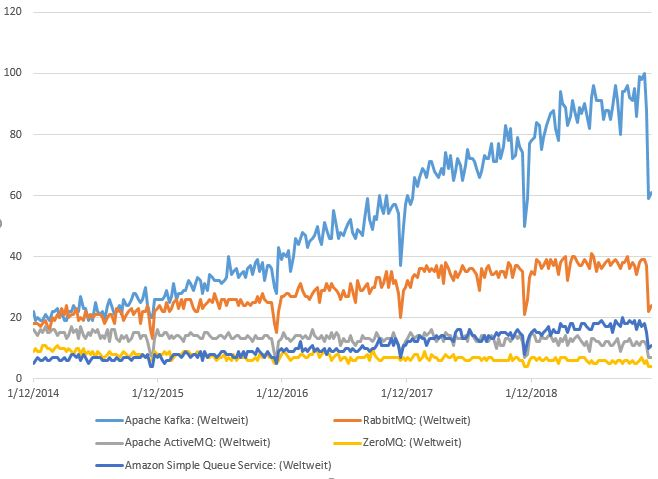
\includegraphics[width=.8\textwidth]{figures/searchinterest.JPG}
	\caption{Relatives Suchinteresse in 5 Jahren; Quelle: Google Trends}
	\label{searchinterest}
\end{figure}

\subsection{Apache Kafka}

Apache Kafka, erstmals erschienen 2011, ist ein Open Source Projekt zur Verarbeitung
von Datenströmen. Es wurde von der Firma LinkedIn entwickelt und später Teil der
Apache Software Foundation.
Es fokussiert sich auf sogenannte \textit{Streams} von Daten, also die Speicherung
und Verarbeitung von Datenströmen. Zwar war Messaging nicht das Hauptziel bei
der Entwicklung Kafkas, allerdings findet es große Verbreitung hierfür.
Kafka bietet vereinfachte Skalierbarkeit durch Clustering. Diese Cluster können sich
über mehrere physische Computer erstrecken \cite{ApacheKa84:online}.

Kafka basiert auf einem simplen Topic-Routing und umfasst
eine Queue, in der Messages gespeichert werden.
Consumer können zusätzlich zum gewöhnlichen Publish-Subscribe Pattern die Nachrichten
auch im Nachhinein noch beliebig aus der Queue abrufen.
Dabei wird intern jede Nachricht an eine sogenannte \textit{Partition} angehängt.
Dies ist nichts anderes als eine Queue mit einer FIFO-Konfiguration, allerdings
wird während des Clustering unter Umständen eine identische Queue mehrmals
vorgehalten. Auch kann es vorkommen, dass eine Partition für einen physischen
Host zu groß wird, und auf mehrere Hosts aufgeteilt wird.
Auf diese Weise ist Kafka sehr gut skalierbar.
Weiter umfasst Kafka nicht nur APIs für Producer und Consumer, sondern auch für
Streams. Diese können von Anwendungen zum Transformieren gesamter Streams verwendet
werden, beispielsweise um von einem Topic nach Verarbeitung der Daten diese direkt
an ein anderes Topic weiterzugeben. \cite{ApacheKa84:online}

Kafka ist in Scala implementiert und läuft auf der Java Virtual Machine. Somit
ist eine gewisse Plattformunabhängigkeit beim Hosting gegeben. Zum Aufsetzen und
Administrieren wird jedoch ZooKeeper, eine weitere Software der Apache Foundation,
benötigt. Dabei kann die Provision, Replikation und Konfiguration aller
Kafka-Instanzen ausschließlich über Zookeeper ablaufen. Im Vergleich zu RabbitMQ
ist der Aufwand einer Installation bei weniger Instanzen hierbei höher, allerdings
vereinfacht Zookeeper dafür die Administration von sehr vielen Instanzen.
Der offizielle Client ist ebenfalls nur für Java/Scala verfügbar, es
gibt jedoch eine Reihe an Drittanbieterbibliotheken, die von Apache empfohlen werden.
Die Kompatibilität ist in Tabelle \ref{compability:table} dargestellt.
Kafka unterstützt das verbreitete AMQP-Protokoll nicht. Es setzt stattdessen
auf eine Eigenentwicklung. Ist die Unterstützung also eine harte Anforderung,
muss auf Drittanbieterbibliotheken zurückgegriffen werden, wobei man wiederum
Performanceverluste, Kompatibilitätsprobleme usw. in Kauf nehmen muss. \cite{KafkaClients:online,ApacheKa84:online}

\paragraph{Routing}
Wie bereits erwähnt, basiert das Routing von Kafka auf Topics. Hierbei sind
zahlreiche Konfigurationen für einzelne Topics möglich.
Unter anderem kann konfiguriert werden, wie lange Nachrichten vorgehalten
werden, wie viel Speicher für sie reserviert wird, ihre maximale Länge, uvm.

Die versendeten Nach\-rich\-ten bestehen aus \textit{key}, \textit{value} und einem
Zeitstempel. Sie enthalten nicht die Partition, in der sie veröffentlicht werden.
Bei beispielsweise einer Partition pro Topic versendet stattdessen der Producer
die Nachrichten direkt an eine Partition.
\paragraph{Besonderheiten}
Bei klassischen Publish-Subscribe Message Brokern ist es unüblich, dass
Nach\-rich\-ten vorgehalten werden und mehrmals abgerufen werden können. Dies
wird jedoch durch die Verwendung einer Queue ermöglicht. Das kann bei der
Verwendung von Kafka als MOM tatsächlich auch zu weiteren Vorteilen führen.
Beispielsweise gibt es so keinen architekturbedingten Nachrichtenverlust, wenn Clients
ausfallen. Diese können die Bearbeitung der Nachrichten dank der Queue zu einem
späteren Zeitpunkt fortsetzen.

Des Weiteren besitzt Kafka APIs, die gezielt Import und Exporte zu Big-Data
Speichersystemen unterstützen. Davon profitieren Systeme, die sehr große Datenmengen
verarbeiten und kommunizieren müssen, wie im Szenario von Event Sourcing.

\paragraph{Analyse nach Eigenschaftenkatalog}
Kafka ist \textbf{at least once} zuzuordnen, wenn es um
Zustellungsgarantien geht. Da die Consumer Nachrichten selbstständig und auch
mehrfach abrufen können, ist davon auszugehen, dass Kafka nicht in die Gruppen
\textit{at most once} oder \textit{exactly once} eingeordnet werden kann. \cite{ApacheKa84:online}

Aufgrund von Kafka's Partitionen liegt eine \textbf{partitioned ordering}
Garantie vor. Zwar ist in den einzelnen Partitionen eine absolute Ordnung, allerdings
kann beispielsweise bei Topic-basierter Partitionierung eine spätere Nachricht
in einem selten gebrauchten Topic weiter vorne stehen als eine frühere in einem
größeren Topic.
Durch die Partitionen wird eine Replikation von Kafka vereinfacht. Hinzu kommt
eine einfache Skalierbarkeit mit Zookeeper. Im Detail wird
pro Cluster, also einer Menge von zusammenarbeitenden Kafka-Instanzen, manuell ein
Anführer bestimmt, der dann alle Entscheidungen über Verteilung von Replikationen
von Partitionen über die Instanzen trifft. Dies bewirkt, dass bei Ausfall einer
Instanz immer noch ein Replika übernehmen kann. \cite{ApacheKa84:online}

Gerade im Bereich Durchsatz kann Kafka jedoch besonders glänzen. Da die Queue und
Routing simpel gehalten sind, werden sehr hohe Durchsätze erreicht.
Dabei wirkt sich die Anzahl an Partitionen indirekt proportional auf den Durchsatz aus.
Es gibt mehrere Benchmarks, die die Performance von Kafka belegen.
Grundsätzlich sind Schreibraten von ungefähr 2.000.000 Nachrichten pro Sekunde
auf durchschnittlicher Hardware möglich. Allerdings ist die Latenz von Kafka
nicht stabil \cite{Linkedin:online, dobbelaere2017kafka}.
\paragraph{Zuordnung zu Use Cases}
Aufgrund der beschriebenen architekturellen Gegebenheiten Kafkas ist dieses für
einige Use Cases besonders geeignet, für andere dafür eher weniger.
Beispielsweise sollte das System keine hohen Anforderungen an das Routing mit sich bringen,
da dies bei Kafka überaus simpel gehalten ist. Allerdings ergeben sich dadurch immense
Performancegewinne, von denen beispielsweise Microservices oder Event Sourcing Szenarien
sehr profitieren können. Des Weiteren können bei Kafka Nachrichten nachträglich erneut
abgerufen werden, was es stark von anderen Implementierungen abhebt.
Oftmals wird Kafka auch wegen seiner hohen Performance gewählt. Diese liegt im
Bereich des fünffachen von RabbitMQ \cite{dobbelaere2017kafka}.
Da keine AMQP-Unterstützung vorhanden ist, wird man jedoch im Enterprise Umfeld
selten Kafka vorfinden.

\subsection{RabbitMQ}
RabbitMQ ist eine von Pivotal Software entwickelte Message Oriented Middleware,
welche das AMQP Protokoll implementiert. Der Server ist in Erlang geschrieben und
plattformunabhängig. Er unterstützt die in \ref{compability:table} dargestellten
Programmiersprachen. Nicht nur AMQP, sondern auch eine Reihe weiterer Protokolle,
wie etwa das im IoT-Umfeld beliebte MQTT, werden unterstützt \cite{dobbelaere2017kafka}.
Daher eignet sich RabbitMQ besonders in Bereichen, in denen mehrere Protokolle zum
Einsatz kommen, oder AMQP eine harte Anforderung ist.

RabbitMQ verwendet eine Queue. Im Detail werden Nachrichten vom Producer an eine
sogenannte Exchange, welche als Router für Nachrichten fungiert, gesendet.
Diese Exchange entscheidet, an welche Queue die Nachricht weitergeleitet wird.
Dabei basiert die Entscheidung auf vorhandenen Routingregeln. Danach wird die
Nachricht in der Queue solange zwischengespeichert, bis sie zugestellt werden
kann. Anders als bei RabbitMQ werden bereits zugestellte Nachrichten daraufhin
gelöscht. \cite{RabbitMQ:online}

\paragraph{Routing}
Da RabbitMQ AMQP implementiert, können sehr komplexe Routing-Logiken umgesetzt
werden. Dabei ist hauptsächlich Topic-basiertes Routing relevant, da dies leichter mit dem
Routing von Kafka verglichen werden kann.
Hierbei wird ein sogenanntes Multipart-Routing unterstützt: Die Nachrichten
werden mit Topics in der Form \texttt{a.b.c} versehen, welche dann mithilfe
von Wildcards gefiltert werden können. Die Konfigurationsmöglichkeiten sind
hierbei sehr vielfältig. Ferner existiert auch ein inhaltsbasiertes Routing. \cite{RabbitMQ:online}

\paragraph{Besonderheiten}
\begin{figure}
  \centering
  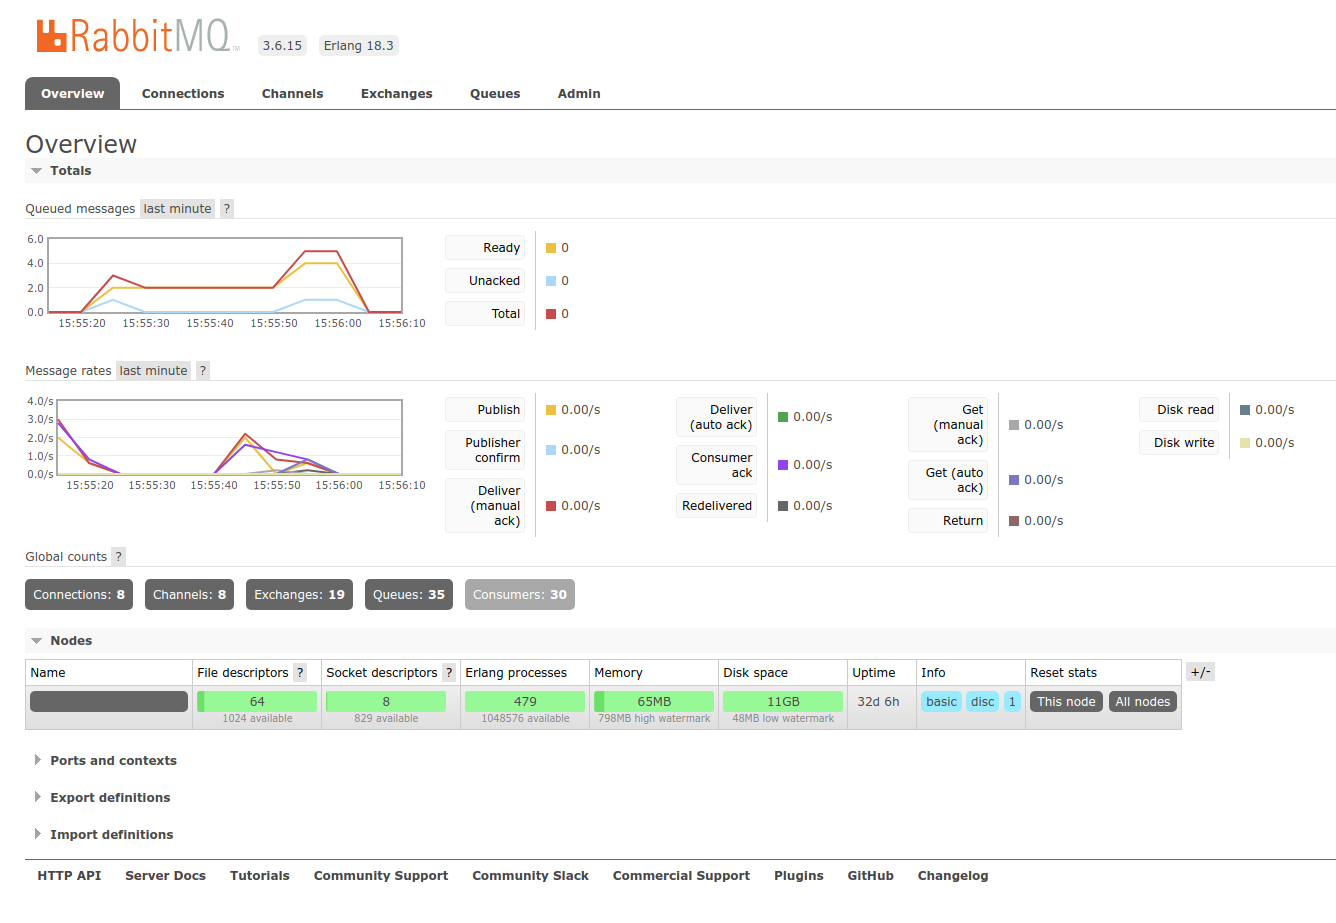
\includegraphics[width=.9\textwidth]{figures/rabbitmq.png}
  \caption{Weboberfläche von RabbitMQ}
  \label{rabbitmq:webinterface}
\end{figure}
RabbitMQ ist von Haus aus mit sehr umfangreichen Monitoring und Management Tools
ausgestattet. Diese erlauben, die meisten wichtigen Aspekte auf einen Blick
zu kontrollieren. In Darstellung \ref{rabbitmq:webinterface} sieht man die Weboberfläche einer RabbitMQ
Instanz, die aktiv verwendet wird. Dabei sind Statistiken zur Gesamtlast sichtbar.
Ferner kann RabbitMQ bei Bedarf komplett in-memory, also ohne Nachrichten auf
einer Festplatte zwischenzuspeichern, sondern nur im Arbeitsspeicher, betrieben
werden.

Die Consumer werden von RabbitMQ aktiv protokolliert. So besteht stets
Transparenz, welcher Consumer welche Nachrichten bereits empfangen hat.
Außerdem können Nachrichten pro Queue mit einer Time to Live, also einer
Gesamtdauer, die eine Nachricht im System existieren darf, versehen werden. Dies
macht vor allem im Kontext von Echtzeit-Daten Sinn.

Auch unterstützt RabbitMQ direkte Antworten auf Nachrichten. Bei Bedarf kann auf
eine Nachricht direkt und ohne entsprechende Antwortqueues geantwortet werden.

\paragraph{Analyse nach Eigenschaftenkatalog}
Die von RabbitMQ übernommenen Garantien bezüglich der Zustellung von Nachrichten sind,
wie auch bei Kafka, \textbf{at least once}. Es besteht also Risiko, dass Nachrichten
doppelt gesendet werden, jedoch nicht, dass sie nie gesendet werden.

Anders verhält es sich bei der Sortierung. RabbitMQ unterstützt \textbf{global order}. Die Exchange
übergibt einer Queue stets die Nachrichten in Batches, die vorsortiert sind.
Verliert ein Client also eine Message aus einer Batch, stellt dies RabbitMQ fest,
und kann die einzelne Nachricht erneut senden.
Das Routing kann, wie bereits erwähnt, sehr komplex sein, und es werden neben
Topic basiertem Routing noch weitere Arten unterstützt.

RabbitMQ unterstützt High Availability durch Replikation vollständiger Ex\-changes.
Allerdings ist der damit verbundene Konfigurationsaufwand im Vergleich zu Kafka
erheblich. Ferner kann relativ einfach skaliert werden, indem dem Cluster neue
Instanzen zugefügt werden. Dabei können neue Queues auf der neuen Instanz zum
Master werden, das heißt, die andere Instanz kopiert sie zwar, aber Consumer
verwenden bevorzugt diesen Master. Anders als bei Kafka kann jedoch keine
bereits bestehende Queue eine neue Instanz zu Ihrem Master machen. Somit ist die
Skalierung mit mehr Aufwand als bei Kafka verbunden.
\paragraph{Use Cases}
Aufgrund der beschriebenen Besonderheiten RabbitMQs eignet sich dieses hervorragend
für Anwendungen, die keine extremen Datenmengen verarbeiten müssen. Dank des
sehr fortgeschrittenen Routings von AMQP können leicht Anwendungen mit sehr
vielen Clients bedient werden.

Ein idealer Use Case ist beispielsweise IoT. Sowohl im privaten, wie im
industriellen Umfeld, kann von geringen Latenzen und dem Support des MQTT
Protokolls profitiert werden. Des Weiteren trägt ein fortgeschrittenes
Monitoring zum einfachen Debuggen von Anwendungen bei.
Auch wird RabbitMQ häufig im Enterprise Bereich eingesetzt. Durch die
Unterstützung von mehreren standardisierten Protokollen wird eine Integration in
ein Umfeld mit stark heterogenen Teilnehmern und auch die Anbindung von älteren
Systemen an RabbitMQ begünstigt.

\newpage
\subsection{NSQ}
NSQ ist eine relativ neue Implementierung des Unternehmens bitly, die ähnliche
Möglichkeiten wie eine MOM bietet. Dabei entfällt jedoch eine zentrale Instanz.
Das bedeutet, es gibt keinen Server, mit dem alle Kommunikationspartner verbunden
sind, sondern alle Teilnehmer sind untereinander verbunden.
Damit man diese Verbindungen nicht
verwalten muss, gibt es eine \textit{Service Discovery}. Diese kann andere
Instanzen entdecken und stellt so ein Netzwerk her. Dezentrale Lösungen wie
diese existierten jedoch schon vor NSQ, beispielsweise ZeroMQ.
Der Client sowie die Service Discovery von NSQ sind in Go implementiert. \cite{NSQ:online}

\paragraph{Besonderheiten}
Wie bereits erwähnt, entfällt eine zentrale Instanz, über die die Nachrichten
geleitet werden. Stattdessen startet jeder Teilnehmer eine Service Discovery,
verbindet sich mit dem Netzwerk und kann anschließend Kanälen beitreten
oder auf Topics abonnieren. Wie bereits bei den anderen Lösungen werden
Nachrichten nach dem Publish-Subscribe Pattern durch das Netzwerk propagiert.
Dementsprechend wird eine Queue lokal bei jedem Teilnehmer gehalten.
Kann eine Nachricht nicht direkt in das Netzwerk eingespeist werden, wird
sie hier gespeichert.
NSQ kann zusätzlich zu den unterstützten Clientbibliotheken (vermerkt in
\ref{compability:table}) eine HTTP-API anbieten, wodurch es auch in anderen
Sprachen genutzt werden kann. Des Weiteren bietet es eine einfache Integration
eines Monitoring sowie eine Weboberfläche zur Administration an. \cite{NSQ:online}
\paragraph{Analyse}
NSQ unterstützt kein standardisiertes Protokoll, es setzt auf eine
Eigenlösung. Architekturbedingt werden Nachrichten ohne jegliche
Ordnungsgarantie, dafür aber \textbf{at least once} übertragen. Eine Skalierbarkeit
durch Replikation entfällt, da für jeden Teilnehmer eine eigene Instanz
gestartet wird. Dank der minimalen Architektur wird ein hoher Durchsatz
und eine gleichbleibend niedrige Latenz erreicht. Die Queue kann wahlweise
auf Festplatte oder Arbeitsspeicher gehalten werden, eine Langzeitspeicherung
entfällt. \cite{NSQ:online}

NSQ eignet sich somit nicht für Event Sourcing, da eine Langzeitspeicherung
erforderlich ist. Weil entsprechende Protokolle nicht unterstützt werden, ist es
auch für den IoT-Bereich ungeeignet. Dank hohem Durchsatz und geringer
Latenz bietet sich NSQ für den Einsatz mit Microservices an.
\section{Vergleich}
Wie sich in den letzten Abschnitten gezeigt hat, gibt es einige große
Unterschiede zwischen RabbitMQ und Kafka.
Während RabbitMQ sehr feine Regelungen beim Routing anbietet, spricht die
Performance für Kafka. Allerdings sind die Protokolle nicht standardisiert und
RabbitMQ unterstützt nicht nur AMQP, sondern gleich mehrere Protokolle.
Kafka bietet wiederum eine langfristige Speicherung für Nachrichten.

Während Kafka im Bereich Microservices oder Event Sourcing seine Stärken
ausspielen kann, überzeugt RabbitMQ bei IoT und im Enterprise Bereich.
Doch trotz aller Unterschiede bieten sowohl RabbitMQ als auch Kafka nach wie
vor einen Message Broker an. Dazu im Kontrast steht NSQ repräsentativ für viele
neue Lösungen, die auf eine zentrale Instanz verzichten.
Architekturbedingt kann NSQ allerdings keine Ordnungsgarantien oder
Langzeitspeicherung von Nachrichten bieten. \cite{RabbitMQBenchmark:online, Linkedin:online}

Allerdings gibt es einen Weg, Vorteile Kafkas und RabbitMQs kombiniert zu nutzen.
Beispielsweise kann man RabbitMQ verwenden, und Kafka einzelne Topics speichern
lassen. Hierbei profitiert man von den regulären Eigenschaften RabbitMQs,
allerdings erhält man gleichzeitig bei Bedarf eine verteilte Langzeitspeicherung
für wichtige Daten. Dieses Szenario ist also vorteilhaft, wenn man zwar RabbitMQ
verwenden würde, allerdings eine Langzeitspeicherung zumindest für einzelne Topics
benötigt wird \cite{dobbelaere2017kafka}.

In einem anderen Beispiel könnte man Kafka verwenden, um Nachrichten
entgegenzunehmen, und eine RabbitMQ Instanz pro Topic, um diese gezielter zu
routen. Hierbei profitiert man von dem hohen Durchsatz Kafkas, wobei man
gleichzeitig das fortgeschrittene Routing RabbitMQs verwenden kann. Dabei gehen
Nachrichten nicht verloren, da Kafka sie speichert. Der Aufbau ist also
geeignet, wenn man das Routing RabbitMQs benötigt, aber die Performance
RabbitMQs zu gering ist \cite{dobbelaere2017kafka}.

\newcommand*\rot{\rotatebox{270}}

\begin{table}
	\centering
	\Rotatebox{270}{
		\begin{tabular}{|l|l|l|l|l|}
			\hline
			\textbf{Eigenschaft}        & \textbf{RabbitMQ}         & \textbf{Apache Kafka}    & \textbf{NSQ}        \\ \hline
			Standardisierte Protokolle  & AMQP, MQPP              & -                 & -                   \\ \hline
			Clientbibliotheken          & alle                    & alle              & alle                \\ \hline
			Möglichkeit zur Skalierung  & Replikation             & Replikation       & -                   \\ \hline
			Durchsatz                   & hoch                    & sehr hoch         & sehr hoch           \\ \hline
			Latenz                      & stabil                  & instabil          & stabil              \\ \hline
			Routingoptionen             & Topic, Channel, Content & Topic             & Topic, Channel      \\ \hline
			Zustellgarantien            & at least once           & at least once     & at least once       \\ \hline
			Speicherort                 & RAM                     & Festplatte        & RAM oder Festplatte \\ \hline
			Langzeitspeicherung         & nicht unterstützt       & unterstützt       & nicht unterstützt   \\ \hline
			Ordnungsgarantien           & partitioned order       & partitioned order & no order            \\ \hline
		\end{tabular}
	}
	\caption{Eigenschaftenkatalog Kafka, RabbitMQ, NSQ}
	\label{featurematrix}
\end{table}

Zusammenfassend können in Tabelle \ref{featurematrix} noch einmal die
wichtigsten Vergleichspunkte abgelesen werden. Dargestellt ist der erarbeitete
Eigenschaftenkatalog, ausgefüllt für Kafka, RabbitMQ, und NSQ.

%\insertemptypage

% ------------------------------------------------------------------------------------------------------
% PART III
% ------------------------------------------------------------------------------------------------------
\cleardoublepage
\chapter{Fallstudie}
\label{part:check24}
\section{Ausgangssituation}
Im Rahmen der Arbeit soll wie bereits erwähnt der Eigenschaftenkatalog mithilfe
eines Fallbeispiels evaluiert werden.
Hierbei ist dieses Szenario durch den Firmenbetreuer CHECK24
Versicherungsservice GmbH gegeben.

% Ist Zustand
Diese ist für das \textit{Versicherungscenter}, eine Webanwendung zum
Verwalten und Vergleichen von Versicherungen und Dokumenten, zuständig.
Kunden können hier abgeschlossene Verträge inklusive aller damit verbundenen
Dokumente und Informationen einsehen und sogar selbst Fremdverträge hinzufügen,
um diese dort zu verwalten.
Dabei durchläuft ein Vertrag, sobald er online abgeschlossen oder hinzugefügt
wurde, eine Reihe von Zustandsänderungen. Es können beispielsweise von
Versicherungen Daten angefordert werden, um vorhandene Daten zu ergänzen, oder
Kunden können neue Angaben machen. Auch bei Vertragsverlängerungen oder
Kündigungen ändern sich Daten. Hierbei wird diese Arbeit vollständig von
Microservices erledigt, und basiert teilweise auf Daten und APIs anderer Teams.

Die Microservices laufen hierbei in jeweils ihrem eigenen Dockercontainer.
Ein Dockercontainer ist eine vom Betriebssystem getrennte, virtualisierte
Umgebung, in der eine Anwendung inklusive aller Abhängigkeiten betrieben werden
kann \cite{docker:online}.
Zudem werden für jeden Microservice zwei Instanzen betrieben, und jede Anfrage
durch ein Loadbalancing geroutet. Dabei wird zusätzlich auf Seite der
Microservices verhindert, dass zweimal der gleiche Request verarbeitet wird.

% Neue Anforderungen
Nun möchten die Entwickler und vor allem auch andere Teams in Zukunft
nachverfolgen können, wann welche Änderungen gemacht wurden. Momentan ist dies
nicht möglich, da Verträge ein einfaches Datenbankmodell sind. Zwar gibt es
Datumsfelder beispielsweise für ein Kündigungsdatum, allerdings sind viele
Änderungen im Nachhinein nicht nachvollziehbar. Es wäre nicht nur übersichtlicher
für die Versicherungen, Kundenberater und anderen Teams, wenn man die einzelnen
Änderungen nachvollziehen könnte, es würde auch das Debugging wesentlich
vereinfachen, da man feststellen könnte, an welcher Stelle ein Fehler entstanden
ist.

Daher wird das Vertragsmodell auf Event Sourcing umgestellt werden.
Hierbei wird, wie bereits in Abschnitt \ref{Message Broker:scenarios} erläutert,
jede Änderung als Event-Objekt mit zugehörigem Datum gespeichert.
Danach ist eine Rekonstruktion möglich, da die Änderungen in der richtigen
Reihenfolge hintereinander den aktuellen Zustand ergeben \cite{kleppmann2017designing}. Die Verwendung einer
Message Oriented Middleware ist in diesem Fall ein offensichtlicher Schritt,
da viele einzelne Anwendungen immer wieder Änderungen beitragen, und alle
anderen Anwendungen diese zeitnah erhalten sollen. Daher muss eine konkrete
Implementierung gewählt und integriert werden. Mithilfe der zuvor aufgestellten
Modelle werden nun die Anforderungen erarbeitet und eine Implementierung
empfohlen.

\section{Anforderungsanalyse}
Die beschriebenen Szenarien, Microservices und Event Sourcing, geben schon
einen ersten Hinweis auf eine geeignete Implementierung.
Um allerdings den vorhin aufgestellten Eigenschaftenkatalog optimal zu
verwenden, sollten zunächst die Anforderungen im Detail analysiert werden.

In Bezug auf Zustellgarantien sind folgende Beobachtungen zu machen. Da teilweise
wichtige Kundendaten bzw. Änderungen daran kommuniziert werden, darf auf keinen
Fall eine Nachricht verloren gehen. \textit{At least once} scheint angebracht zu
sein. Eine Wiederholung von Nachrichten sollte jedoch eingeplant werden und wird zu
zusätzlichem Implementierungsaufwand führen. Da jedoch die Events üblicherweise
mit einem Timestamp versehen sein werden, sollte ein Filter bei den Clients
trivial sein, da davon ausgegangen werden kann, dass keine zwei Änderungen
gleichen Inhalts in der gleichen Millisekunde stattfinden.

Da Events im Nachhinein abgerufen werden müssen, um den aktuellen Zustand zu
berechnen, muss die Implementierung eine Queue mit permanenter
Speichermöglichkeit anbieten.
Eine Ordnung der Nachrichten ist in diesem Szenario keine Primäranforderung. Zwar
wäre es schlecht, wenn eine Nachricht über eine Änderung einer Versicherung vor der
Nachricht über ihre Erstellung ankommt, allerdings wird keine \textit{total order}
benötigt. Da bei der Erstellung der Events ein Zeitstempel abgespeichert wird,
kann die korrekte Abfolge von Events auch im Nachhinein noch rekonstruiert werden.

Da das Versicherungscenter ein wachsender Geschäftszweig der CHECK24-Gruppe ist,
ist Skalierung eine große Herausforderung. Eine einfache Lösung, die auch Mittel für
Hochverfügbarkeit mit sich bringt, ist gewünscht. Ebenso ist in naher Zukunft
mit hohen Lasten zu rechnen. Eine MOM kann hierbei unabhängig vom restlichen
System skaliert werden, da die Microservices eine Mehrfachbearbeitung von
Nachrichten verhindern. So können beliebig viele Instanzen eines Services die
gleiche Nachricht empfangen, ohne dass es zu Problemen kommt.
So wird für eine MOM eine unabhängige Skalierung ermöglicht.

Ein fortgeschrittenes Routing wird nicht benötigt. Da die Kommunikation 
bisher über ein Datenbankmodell bzw. über HTTP-Calls erfolgte, werden keine
komplexen Routen verwendet. Das primäre Ziel ist, die momentane Lösung durch eine
zukunftstauglichere zu ersetzen, nicht den Funktionsumfang zu erweitern. Da
außerdem die Middleware nur von einem Team und momentan ca. 100 Microservices
verwendet wird, ist das Routing trivial.

Eine stabile Latenz ist teilweise wichtig.
Für einen Kunden macht es keinen großen Unterschied, ob er die Vertragsdokumente,
die eine Versicherungsgesellschaft bereitgestellt hat, einige Millisekunden
später sieht. Ebenso verhält es sich bei der Kündigung oder der
Abschlussbestätigung seitens der Versicherung.
Es verhält sich allerdings anders, sobald der Kunde seine Verträge betrachtet.
Wird der aktuelle Vertragszustand aus allen Events berechnet, und dauert dies
sehr lange, so muss der Kunde auch länger darauf warten. Daher sollte in dieser
Hinsicht eine stabile Latenz gewährleistet sein.

Hinsichtlich einer Queue ist eine langfristige Speichermöglichkeit
wünschenswert. Eventuell können zu einem späteren Zeitpunkt Caching-Lösungen
implementiert werden, oder der Verlauf ist für Verträge eines gewissen Alters
nicht mehr relevant. Dies kann allerdings erst in der Zukunft abgewogen werden.
Bis dahin sollten keinesfalls Verträge gelöscht werden, die noch nicht permanent
in einer anderen Speicherlösung abgelegt wurden.
Da für solche Datenmengen die Speicherung im Arbeitsspeicher sehr teuer werden
kann und die Geschwindigkeit ausreicht, genügt die Speicherung auf Festplatte.

Somit sind die in Abschnitt \ref{formal} erarbeiteten
Kriterien betrachtet und nach ihrer Wichtigkeit beurteilt worden. Dieses Ergebnis
ist nochmals in Tabelle \ref{requirementsmatrix} festgehalten.

\begin{table}[b]
	\centering
	\begin{tabular}{|l|l|}
		\hline
		\textbf{Eigenschaft}      & \textbf{Anforderung?}              \\ \hline
		Standardisierte Protokolle & nein                               \\ \hline
		Clientbibliotheken & Javascript \\ \hline
		Möglichkeit zur Skalierung & unabhängig \\ \hline
		Hoher Durchsatz           & ja \\ \hline
		Stabile Latenz            & teilweise ja \\ \hline
		Routing & Topic ausreichend \\ \hline
		Zustellgarantien           & \textit{at least once} ausreichend \\ \hline
		Speicherort               & Festplatte bevorzugt               \\ \hline
		Langzeitspeicherung       & ja                   \\ \hline
		Ordnungsgarantien          & partitioned                        \\ \hline
	\end{tabular}
	\caption{Anforderungstabelle CHECK24 Versicherungsservice GmbH}
	\label{requirementsmatrix}
\end{table}

\section{Empfehlung}
Aufgrund der im vorhergehenden Abschnitt aufgestellten Anforderungen kann nun
eine Empfehlung ausgesprochen werden.
Die Punkte deuten fast ausschließlich auf Apache Kafka hin.
Es eignet sich sehr gut, um eine Microservice-In\-fra\-struk\-tur wie die oben
beschriebene zu betreiben. Zudem eignet es sich dank der Langzeitspeicherung für
Event Sourcing.
Werden Änderungen an Verträgen gemacht, können diese als Message in Kafka
abgelegt werden, und Worker können diese dann stückweise abarbeiten, bzw. andere
Anwendungen diese abrufen und sind damit immer auf dem neuesten Stand.
Somit eignet sich in diesem Szenario Kafka besser als RabbitMQ. Eine
Erweiterung um die Routing-Kapazitäten RabbitMQs ist vorerst nicht notwendig.
Es entfällt also auch eine Erweiterung um das Routing von RabbitMQ.

Allerdings ergeben sich mit Kafka auch Nachteile. Beispielsweise ist wie
bereits erwähnt das Hosting nicht trivial. Es werden Zookeeper bzw.
eine Sammlung von Skripten verwendet, um Kafka zu administrieren.
Auch würde dies eine Abweichung zum sonstigen Hosting bedeuten,
da die Microservices alle in sauber getrennten, eigenen Dockercontainern
betrieben werden.
Dem Problem kann jedoch entgegengewirkt werden, indem man Kafka auch
in einem Dockercontainer betreibt. Hierbei sollte bei der Skalierung dafür
gesorgt werden, dass mindestens zwei verbundene Instanzen auf mehr als
einem physischen Server laufen.

Des Weiteren werden mit Kafka keine stabilen Latenzen erreicht
\cite{Linkedin:online}. Dies kann zu
Problemen führen, wenn ein Kunde seine Vertragsdaten im Frontend betrachtet.
Hierbei werden vom zugehörigen Microservice die Daten bereitgestellt. Braucht
dieser also zu lange, um alle Events für einen Vertrag abzurufen, muss der
Kunde länger warten.

Dieses Problem kann auf zwei Arten gelöst werden.
Beispielsweise kann der aktuelle Zustand in einer Datenbank mitgeführt werden.
Bei einem Änderungsevent muss so nur ein simpler Microservice diesen Eintrag
des jeweils aktuellen Zustands aktualisieren. Auf diese Weise können
Microservices, die den aktuellen Zustand eines Vertrags benötigen, diesen sehr
schnell abrufen.
Der Aufwand hierfür ist gering, besagte Microservices
können weiterhin aus der bereits existierenden Datenbank abfragen, und ein
simpler Microservice, der bei Change Events diese updated, ist dank der MOM
schnell integriert. Somit kann trotz instabiler Latenzen Kafka verwendet werden.

Die zweite Lösung wäre, RabbitMQ aufgrund seiner geringen Latenzen zu verwenden,
und die Speicherung der Events in einer externen Datenbank vorzunehmen.
Hierbei würde man von der erleichterten Administration von RabbitMQ profitieren,
und gleichzeitig eine ausreichend schnelle Langzeitspeicherung selbst
hinzufügen. Allerdings wäre der Gesamtaufwand wesentlich höher, als der Aufwand
der vorherigen Lösung. Dies würde also nur in Frage kommen, wenn eine
langfristige Speicherung von Events in Kafka ungeeignet ist und der Mehraufwand
in Kauf genommen werden kann.

Die Empfehlung fällt auf Kafka. Hiermit können mit geringem Aufwand die Anforderungen
befriedigt werden. Unzureichend erfüllte Anforderungen können ebenfalls einfach
erfüllt werden. Andere Lösungen sind möglich, stellen jedoch einen erheblichen
Mehraufwand dar.

%\insertemptypage

% ------------------------------------------------------------------------------------------------------
% PART IV
% ------------------------------------------------------------------------------------------------------
\cleardoublepage
\chapter{Schluss}
\label{part:end}
\section{Fazit}
In dieser Arbeit wurden die Grundlagen von Message Oriented Middlewares
beleuchtet. Dabei wurden der allgemeine Aufbau und die Funktion
einzelner Komponenten erklärt. Vor- und Nachteile einer MOM wurden
abgewägt.
Es wurden außerdem einige praxisnahe Szenarien, in denen oft eine Message
Oriented Middleware Einsatz findet, aufgezeigt. Hierbei wurde erklärt,
warum sie jeweils von dieser Verwendung profitieren.

Davon ausgehend wurde ein Eigenschaftenkatalog erarbeitet,
mithilfe dessen eine erleichterte Analyse verschiedener Implementierungen
ermöglicht wurde. Dieser umfasst die in der Praxis wichtigen Kriterien,
in denen sich Implementierungen unterscheiden können. Dabei wurde jede
dieser Eigenschaften verständlich begründet, sodass selbst fachfremde
sie verwenden können, um eine Auswahl zu treffen.

Anschließend wurden die verbreiteten Implementierungen analysiert und
miteinander auf Grundlage dieses Eigenschaftenkatalogs verglichen.
Zusätzlich wurde eine grundsätzlich verschiedene Neuentwicklung analysiert.
Hierdurch wurde gezeigt, dass der Katalog anwendbar ist
und auch für zukünftige Implementierungen genutzt werden kann.

Zur Validierung des Eigenschaftenkatalogs wurde dieser abschließend auf ein
praktisches Szenario angewendet. Eine Integration in den durch die CHECK24
Versicherungsservice GmbH gegebenen Anwendungsfall wurde geplant und in
allen Punkten des Katalogs untersucht. Anschließend wurde eine Empfehlung
ausgesprochen. Diese wurde auch vom Rest des Teams nach gemeinsamer Analyse
getragen.

Die Arbeit informiert ausführlich über die führenden Implementierungen,
gibt jedoch gleichzeitig ein Werkzeug mit an die Hand, mit dem Neuentwicklungen
eingeordnet werden können. Wie demonstriert wurde, kann sie als Grundlage
für Entscheidungen in echten Anwendungsfällen dienen.

\section{Ausblick}
Eine Message Oriented Middleware findet in vielen modernen Systemen Anwendung.
Eine sauber getrennte, asynchrone, und vor allem performante
Kommunikationslösung für Softwaresysteme wird auch in nächster Zukunft aus den
meisten Systemen nicht wegzudenken sein.
Dabei wächst das Angebot an Lösungen stetig. Die Spezialisierung der einzelnen
Lösungen ist dabei hoch, die meisten Neuentwicklungen sind auf einen bestimmten
Anwendungsfall zugeschnitten.
Somit wäre es sicher interessant, den Vergleich dieser Arbeit auf weitere
Implementierungen auszuweiten. Diese werden sich jedoch untereinander weniger
stark unterscheiden als Kafka und RabbitMQ.

Auch die neueste Entwicklung - Brokerlose MOMs - könnten mit den erarbeiteten
Metriken leicht eingeschätzt werden, auch wenn ihre detaillierte Behandlung
den Rahmen der Arbeit gesprengt hätte.
Diese Entwicklung lohnt es sich jedoch in jedem Fall zu verfolgen.
Dabei gibt es andere Mechanismen zu erforschen und optimieren, wie beispielsweise
die zwingend notwendige Service Discovery, mit der solche Peer to Peer Systeme
funktionieren. Da diese Entwicklungen noch relativ neu sind, wird hier in den
nächsten Jahren noch viel weiterentwickelt werden.

RabbitMQ sticht mit seinen Enterprise Eigenschaften hervor, aufgrund derer es
trotz vergleichsweise niedrigem Durchsatz immer noch große Verbreitung findet.
Ob RabbitMQ in naher Zukunft von einer anderen Implementierung abgelöst werden
kann, die einen ähnlichen Support für viele Protokolle anbietet, bleibt
spannend. Ebenso wäre eine Entwicklung interessant, die neue Architekturen,
wie Peer to Peer MOMs, in Verbindung mit dem Support für standardisierte
Protokolle bringt. Dies wäre beispielsweise für den IoT-Bereich relevant.

Es lässt sich abschließend sagen, dass in den nächsten Jahren sicher noch viel
auf dem Gebiet der Message Oriented Middleware passieren wird. Diese Arbeit hat
eine Übersicht über den aktuellen Stand der Entwicklung gegeben, während die
verwendeten Methoden auch in der Zukunft verwendet werden können.

%\insertemptypage

% ------------------------------------------------------------------
% VERZEICHNISSE
% ------------------------------------------------------------------

\chapter*{Anhang}
\label{ch:annex}

% Literaturverzeichnis
\cleardoublepage
% \nocite{*}
\printbibliography
% Abk�rzungen

\cleardoublepage
\printglossaries

% Abbildungsverzeichnis
\cleardoublepage
\listoffigures

% Tabellenverzeichnis
\cleardoublepage
\listoftables

%% Optionale Verzeichnisse -- bei Bedarf einkommentieren
% Listingsverzeichnis
%\cleardoublepage
%\lstlistoflistings

% Algorithmenverzeichnis
%\cleardoublepage
%\listofalgorithms

% ------------------------------------------------------------------
% ANHANG
% ------------------------------------------------------------------

% \cleardoublepage
\include{appendix}
\end{document}
